%!TEX TS-program = xelatex
% CUHKthesis @ https://github.com/zfengg/CUHKthesis
%
%	A simple tex template for the thesis at CUHK.
%
% Author: Zhou Feng @ 15/12/2022
% ---------------------------------------------------------------------------- %
%                                   preamble                                   %
% ---------------------------------------------------------------------------- %
\documentclass[12pt]{report}
% ---------------------------- settings & commands --------------------------- %
% !TEX root = ../thesis.tex
% packages
\usepackage{amsmath,amsfonts,amssymb}
\usepackage{mathrsfs}
\usepackage{mathtools}
\usepackage{caption}
\usepackage[shortlabels,inline]{enumitem}
\usepackage{booktabs}  % for professional tables

% figure
\usepackage{tikz}
\usepackage{tikz-cd}
\usepackage{float}
\usepackage{graphicx}
\DeclareGraphicsExtensions{.pdf,.png,.jpg,.jpeg}
\graphicspath{ {figures/}{figures/DefectGPT/}{figures/Framework/}{figures/Med/}{figures/UAV/} }

% layout
\footskip 4.ex
\renewcommand{\baselinestretch}{1.5}
\usepackage[a4paper,inner=4cm,outer=2.5cm]{geometry}

% Chinese
\usepackage[scheme=plain]{ctex}
%\usepackage{xeCJK} % Chinese via xelatex
%\setCJKmainfont{SimSun}
% \setCJKsansfont{SimSun}
% \setCJKmonofont{SimSun}

% ------------------------------ reference style ----------------------------- %
\usepackage[numbers,sort]{natbib} 	% automatically sort the citations
%\renewcommand\bibname{Bibliography}

% ------------------------------ footer & header ----------------------------- %
% \usepackage{fancyhdr}
% % def headstyles
% \newcommand{\headstyle}{%
% 	\fancyhead[L]{}
% 	\fancyhead[C]{}
% 	\fancyhead[R]{}
% }
% % def footstyles
% \makeatletter
% \newcommand{\footstyle}{%
% 	\fancyfoot[L]{}
% 	\fancyfoot[C]{\thepage}
% 	\fancyfoot[R]{}
% }
% \newcommand{\authorfootstyle}{%
% 	\fancyfoot[L]{}
% 	\fancyfoot[C]{\thepage}
% 	\fancyfoot[R]{}
% }
% \makeatother
% % set global pagestyle
% \pagestyle{fancy}
% \fancyhf{} % clear the orginal headfoot style
% \headstyle
% \footstyle
% % def first-page pagestyle
% \fancypagestyle{firstpage}{%
% 	\fancyhf{}
% 	\headstyle
% 	\authorfootstyle
% }
% % def main pagestyle
% \fancypagestyle{main}{%
% 	\fancyhf{}
% 	\headstyle
% 	\footstyle
% }
%\renewcommand{\headrulewidth}{0pt}
%\renewcommand{\footrulewidth}{0.4pt}
%\renewcommand{\headrule}{\rule{\textwidth}{0.4pt}}

% appendix
\usepackage{appendix}

% -------------------------- hyperlinks & bookmarks -------------------------- %
\usepackage{aliascnt} %  \autoref
\usepackage[pdfusetitle,
bookmarks=true,
pagebackref,
colorlinks,
linkcolor=blue,
citecolor=blue,
urlcolor=blue]{hyperref}

% ------------------------------- environments ------------------------------- %
\usepackage{amsthm}
\newtheorem{dummy}{***}[section]

\theoremstyle{plain}
\newaliascnt{theorem}{dummy}
\newtheorem{theorem}[theorem]{Theorem}
\aliascntresetthe{theorem}
\providecommand*{\theoremautorefname}{Theorem}
\newaliascnt{proposition}{dummy}
\newtheorem{proposition}[proposition]{Proposition}
\aliascntresetthe{proposition}
\providecommand*{\propositionautorefname}{Proposition}
\newaliascnt{corollary}{dummy}
\newtheorem{corollary}[corollary]{Corollary}
\aliascntresetthe{corollary}
\providecommand*{\corollaryautorefname}{Corollary}
\newaliascnt{lemma}{dummy}
\newtheorem{lemma}[lemma]{Lemma}
\aliascntresetthe{lemma}
\providecommand*{\lemmaautorefname}{Lemma}
\newaliascnt{conjecture}{dummy}
\newtheorem{conjecture}[conjecture]{Conjecture}
\aliascntresetthe{conjecture}
\providecommand*{\conjectureautorefname}{Conjecture}

\theoremstyle{definition}
\newaliascnt{definition}{dummy}
\newtheorem{definition}[definition]{Definition}
\aliascntresetthe{definition}
\providecommand*{\definitionautorefname}{Definition}
\newaliascnt{example}{dummy}
\newtheorem{example}[example]{Example}
\aliascntresetthe{example}
\providecommand*{\exampleautorefname}{Example}

\theoremstyle{remark}
\newaliascnt{remark}{dummy}
\newtheorem{remark}[remark]{Remark}
\aliascntresetthe{remark}
\providecommand*{\remarkautorefname}{Remark}

\newtheorem{exercise}{Exercise}[section]
\providecommand*{\exerciseautorefname}{Exercise}

% ---------------------------------- autoref --------------------------------- %
\renewcommand{\sectionautorefname}{Section}
\renewcommand{\chapterautorefname}{Chapter}
%\renewcommand{\equationautorefname}{Equation}

% ------------------------------------ misc ----------------------------------- %
\allowdisplaybreaks

% !TEX root = ../thesis.tex
\makeatletter
% ----------------------------------- info ----------------------------------- %
\newcommand{\titlezh}[1]{\gdef\@titlezh{#1}}%
\newcommand{\@titlezh}{\@latex@warning@no@line{No \noexpand\titlezh given}}
\newcommand{\degree}[1]{\gdef\@degree{#1}}%
\newcommand{\@degree}{\@latex@warning@no@line{No \noexpand\degree given}}
\newcommand{\programme}[1]{\gdef\@programme{#1}}%
\newcommand{\@programme}{\@latex@warning@no@line{No \noexpand\programme given}}
\newcommand{\institution}[1]{\gdef\@institution{#1}}%
\newcommand{\@institution}{\@latex@warning@no@line{No \noexpand\institution given}}
\newcommand{\committee}[1]{\gdef\@committee{#1}}%
\newcommand{\@committee}{\@latex@warning@no@line{No \noexpand\committee given}}

% ----------------------------------- pages ---------------------------------- %
% coverpage
\renewcommand{\maketitle}{%
	\thispagestyle{empty}
	\pdfbookmark{Titlepage}{titlepage}
	\vspace*{5mm}
	\begin{center}
	\Large{ \bf \@title}
	\end{center}
	\vspace*{20mm}
	
	\begin{center}
	\@author
	\end{center}
	\vspace*{20mm}

	\begin{center}
	A Thesis Submitted in Partial Fulfilment \\
	of the Requirements for the Degree of \\
	\@degree \\
	in \\
	\@programme
	\end{center}
	\vspace*{20mm}

	\begin{center}
	\@institution \\
	\@date
	\end{center}

	\clearpage
	\thispagestyle{empty}
	\vspace*{60mm}
	\begin{center}
		\underline{Thesis Assessment Committee}\\
		\vspace{5mm}
		\@committee
	\end{center}
	\vspace*{50mm}
}

% abstract: english
\newcommand{\makeabstract}{%
	\chapter*{Abstract}
	\addcontentsline{toc}{chapter}{Abstract}
%	\vspace{0.5cm}
	% !TEX root = ../thesis.tex

This research aims to address the fundamental "cognitive-physical gap" faced by Large Language Models (LLMs) when applied to physical world decision-making. To tackle this challenge, we propose and plan to implement a novel Agent architecture named CORTEX.

\textbf{Background and Problem Statement:} While Large Language Models have achieved tremendous success in textual reasoning, they exhibit a fundamental cognitive-physical gap when applied to tasks requiring interaction with dynamic physical environments. This gap stems from LLMs' training on static text corpora, lacking contextualized understanding of real-time physical states, resulting in internal world models that are disconnected from physical reality.

\textbf{Research Objectives and Methodology:} The core contributions of this research span three levels: 1) Theoretical level: we propose to construct a "Three-Layer Digital Twin Decision Framework" (L1-Descriptive, L2-Predictive, L3-Interactive), providing a theoretical foundation for systematically evaluating physical world AI; 2) Architectural level: we plan to design the CORTEX architecture, which systematically addresses three major challenges of LLMs in the physical world—reality grounding, model utilization, and safe execution—through deep extensions of RAG and Agent paradigms; 3) Empirical level: we propose a quantitative evaluation method for "cognitive gains" and plan to validate the framework through three representative cases corresponding to L1, L2, and L3 respectively.

\textbf{Research Progress and Implementation Plan:} The CORTEX architecture is based on a cognitive science-inspired four-stage loop: 1) Perceptual Grounding \& Context Formulation, 2) Causal Inference \& Predictive Simulation, 3) Action Policy Generation \& Validation, and 4) Physical Interaction \& Model Calibration. To validate this architecture's effectiveness across diverse domains, this research employs a multi-case study approach.

\textbf{Completed Work:} The first case study in \textit{predictive decision-making for building health monitoring} has been successfully completed. This work developed and validated a Digital Twin that fuses Building Information Modeling (BIM) data with real-time sensor time-series data, demonstrating that the CORTEX architecture can significantly enhance maintenance decision quality and reduce false positive rates by 35\% compared to traditional approaches.

\textbf{Ongoing Work:} Two additional case studies are currently underway. The second case study focuses on \textit{assistive decision-making in medical ultrasound diagnosis (cancer treatment planning)}, planning to implement a non-visual Digital Twin based on feature extraction from 2D ultrasound images. The third case study addresses \textit{autonomous decision-making in UAV exploration}, proposing to utilize real-time 3D point cloud data to construct Digital Twins for navigation and obstacle avoidance in unknown environments.

\textbf{Expected Outcomes and Contributions:} Upon completion, this research is expected to quantitatively validate that the CORTEX architecture significantly enhances the quality, robustness, and safety of LLM-driven decisions across diverse physical interaction tasks. The main contributions include: (1) a theoretical framework bridging LLM reasoning and physical world interaction, (2) practical implementation methodology for Digital Twin-enhanced cognitive architectures, (3) empirical validation across three distinct domains, and (4) deployment guidelines for such systems in real-world applications.

The expected outcomes of this research will provide a validated, scalable architectural blueprint for developing more powerful and reliable physical world artificial intelligence systems, advancing next-generation AI systems toward reliable and intelligent interaction with the physical world.
	\clearpage
}

% abstract: chinese
\newcommand{\makeabstractChinese}{%
	\chapter*{摘要}
	\addcontentsline{toc}{chapter}{摘要}
%	\vspace{0.5cm}
	% !TEX root = ../thesis.tex

本研究旨在解决大型语言模型(LLM)在应用于物理世界决策时面临的根本性"认知-物理鸿沟"。尽管LLM在文本推理方面取得巨大成功,但在需要与动态物理环境交互的任务中,由于基于静态文本语料库训练而缺乏对实时物理状态的情境化理解,导致其内部世界模型与物理现实脱节。

为应对此挑战,本研究提出并计划实现名为CORTEX的新型Agent架构。研究的核心贡献体现在三个层面:理论层面构建"三层数字孪生决策框架"(L1-描述性,L2-预测性,L3-交互式),为系统性评估物理世界AI提供理论基座;架构层面设计CORTEX架构,通过深度扩展RAG和Agent范式,系统性解决LLM在物理世界中的现实接地、模型利用和安全执行三大挑战;实证层面提出"认知增益"量化评估方法,通过三个分别对应L1、L2、L3的代表性案例进行验证。

CORTEX架构基于认知科学启发的四阶段循环:感知接地与情境构建、因果推理与预测仿真、行动策略生成与验证、物理交互与模型校准。为验证该架构在不同领域的有效性,本研究采用多案例研究方法。建筑健康监测的预测决策案例研究已成功完成,开发并验证了融合建筑信息模型数据与实时传感器时序数据的数字孪生,证明CORTEX架构能够显著提升维护决策质量。

目前正在开展两个额外案例研究:医疗超声诊断中的辅助决策,计划实现基于2D超声图像特征提取的非视觉数字孪生;无人机探索中的自主决策,拟利用实时3D点云数据构建数字孪生进行未知环境导航和避障。研究完成后,预期将定量验证CORTEX架构在多样化物理交互任务中显著提升LLM驱动决策的质量、鲁棒性和安全性。本研究成果将为开发更强大、更可靠的物理世界人工智能系统提供经过验证的、可扩展的架构蓝图。
	\clearpage
}

% acknowledgement
\newcommand{\makeacknowledgement}{%
	\chapter*{Acknowledgement}
	\addcontentsline{toc}{chapter}{Acknowledgement}
	% !TEX root = ../thesis.tex

I am grateful to my supervisor Professor $ X $.
	\clearpage
}

% update toc
\newcommand{\addloftotoc}{%
	\cleardoublepage
	\phantomsection
	\addcontentsline{toc}{chapter}{\listfigurename}
}

\newcommand{\addlottotoc}{%
	\cleardoublepage
	\phantomsection
	\addcontentsline{toc}{chapter}{\listtablename}
}

\newcommand{\addbibtotoc}{%
	\phantomsection
	\addcontentsline{toc}{chapter}{\bibname}
}

% add bookmark
\newcommand{\addtocbm}{%
	\cleardoublepage
	\pdfbookmark{\contentsname}{toc}
}

\makeatother
% !TEX root = ../thesis.tex
% -------------------------------- fast-typing ------------------------------- %
% cali characters
\newcommand{\calF}{\mathcal{F}}
\newcommand{\calB}{\mathcal{B}}
\newcommand{\calP}{\mathcal{P}}
\newcommand{\calT}{\mathcal{T}}
\newcommand{\calD}{\mathcal{D}}
\newcommand{\calQ}{\mathcal{Q}}
\newcommand{\calR}{\mathcal{R}}
\newcommand{\calM}{\mathcal{M}}
\newcommand{\calL}{\mathcal{L}}
\newcommand{\calI}{\mathcal{I}}
\newcommand{\calG}{\mathcal{G}}
\newcommand{\calW}{\mathcal{W}}
% scurf characters
\newcommand{\scrB}{\mathscr{B}}
\newcommand{\scrD}{\mathscr{D}}
\newcommand{\scrP}{\mathscr{P}}
\newcommand{\scrA}{\mathscr{A}}
\newcommand{\scrE}{\mathscr{E}}
\newcommand{\scrC}{\mathscr{C}}
\newcommand{\scrT}{\mathscr{T}}
\newcommand{\scrQ}{\mathscr{Q}}
\newcommand{\scrF}{\mathscr{F}}
\newcommand{\scrG}{\mathscr{G}}
\newcommand{\scrW}{\mathscr{W}}
% blackboad characters
\newcommand{\bbQ}{\mathbb{Q}}
\newcommand{\bbR}{\mathbb{R}}
\newcommand{\bbC}{\mathbb{C}}
\newcommand{\bbZ}{\mathbb{Z}}
\newcommand{\bbN}{\mathbb{N}}
\newcommand{\bbP}{\mathbb{P}}
\newcommand{\bbT}{\mathbb{T}}
% frak characters
\newcommand{\frX}{\mathfrak{X}}
% rome characters
\newcommand{\rmN}{\mathrm{N}}
\newcommand{\rmR}{\mathrm{R}}
% math operators
\DeclareMathOperator*{\Lim}{Lim}
\DeclareMathOperator*{\llim}{\underline{lim}}
\DeclareMathOperator*{\ulim}{\overline{lim}}
\DeclareMathOperator*{\essinf}{ess\,inf}
\DeclareMathOperator*{\esssup}{ess\,sup}
\DeclareMathOperator*{\intersect}{\cap}
\DeclareMathOperator*{\Intersect}{\bigcap}
\DeclareMathOperator*{\union}{\cup}
\DeclareMathOperator*{\Union}{\bigcup}
\DeclareMathOperator{\ex}{ex}
\DeclareMathOperator{\co}{co}
\DeclareMathOperator{\diam}{diam}
\DeclareMathOperator{\supp}{supp}
\DeclareMathOperator{\Var}{Var}
\DeclareMathOperator{\Exp}{Exp}
\DeclareMathOperator{\Dim}{Dim}
\DeclareMathOperator{\ldim}{\underline{\dim}}
\DeclareMathOperator{\udim}{\overline{\dim}}
% commonly used
\newcommand{\Ndash}{\nobreakdash--}
\newcommand{\sigmaAlg}{$\sigma$\nobreakdash-algebra }
\providecommand{\abs}[1]{\lvert#1\rvert}
\providecommand{\Abs}[1]{\left\lvert#1\right\rvert}
\providecommand{\norm}[2][]{\lVert#2\rVert_{#1}}
\providecommand{\Norm}[2][]{\left\lVert#2\right\rVert_{#1}}
\newcommand{\ndiml}[1][n]{$#1$\nobreakdash-dim}
\newcommand{\padic}{$p$\nobreakdash-adic}
\newcommand{\kOrder}[1]{$#1$\nobreakdash-order}
\newcommand{\mDash}[2]{$#1$\nobreakdash-#2}
\newcommand{\euclid}[1][d]{\mathbb{R}^{#1}}
\newcommand{\innerprod}[2]{\langle #1, #2 \rangle}
\newcommand{\pairing}[2]{\left(#1, #2\right)}
\newcommand{\oneOver}[1]{\frac{1}{#1}}
\newcommand{\energy}[2][s]{I_{#1}(#2)}
\newcommand{\capacity}[2][s]{g_{#1}(#2)}
\newcommand{\wt}[1]{\widetilde{#1}}
\newcommand{\wh}[1]{\widehat{#1}}
\newcommand{\cl}[1]{\overline{#1}}
% dimensions
\newcommand{\dimH}{\dim_{\mathrm{H}}}
\newcommand{\dimP}{\dim_{\mathrm{P}}}
\newcommand{\dimB}{\dim_{\mathrm{B}}}
\newcommand{\dimC}{\dim_{\mathrm{C}}}
\newcommand{\dimF}{\dim_{\mathrm{F}}}
\newcommand{\dimE}{\dim_{\mathrm{e}}}
\newcommand{\dimsub}[1]{\dim_{\mathrm{#1}}}
\newcommand{\uDim}[1]{\overline{\dim}_{\mathrm{#1}}}
\newcommand{\lDim}[1]{\underline{\dim}_{\mathrm{#1}}}
\newcommand{\locDim}[2]{D(#1, #2)}
\newcommand{\ulocDim}[2]{\overline{D}(#1, #2)}
\newcommand{\llocDim}[2]{\underline{D}(#1, #2)}
\newcommand{\uTau}{\overline{\tau}}
\newcommand{\lTau}{\underline{\tau}}
% measures
\newcommand{\leb}[1]{\mathcal{L}(#1)}
\newcommand{\lebRes}[1]{\mathcal{L}\vert_{#1}}
\newcommand{\haus}[2]{\mathcal{H}^{#1}(#2)}
\newcommand{\hausC}[2]{\mathcal{H}^{#1}_{\infty}(#2)}
\newcommand{\hausO}[3]{\mathcal{H}^{#1}_{#2}({#3})}
\newcommand{\Haus}[1]{\mathcal{H}^{#1}}
\newcommand{\HausC}[1]{\mathcal{H}^{#1}_{\infty}}
\newcommand{\HausO}[2]{\mathcal{H}^{#1}_{#2}}
\newcommand{\pack}[2]{\mathcal{P}^{#1}(#2)}
\newcommand{\packP}[2]{\mathcal{P}^{#1}_{0}(#2)}
\newcommand{\packC}[3]{\mathcal{P}^{#1}_{#2}(#3)}
\newcommand{\Pack}[1]{\mathcal{P}^{#1}}
\newcommand{\PackP}[1]{\mathcal{P}^{#1}_{0}}
\newcommand{\PackC}[2]{\mathcal{P}^{#1}_{#2}}
% ----------------------------------- misc ----------------------------------- %

% ----------------------------------- info ----------------------------------- %
\title{THESIS TITLE}
\titlezh{中文标题}
\author{LAST, First}
\degree{Doctor of Philosophy}
\programme{Mathematics}
\institution{The Chinese University of Hong Kong}
\date{December 2022}
\committee{%
	Professor LAST First (Chair)\\
	Professor ZHANG San (Thesis Supervisor)\\
	Professor LI Si (Thesis Co-supervisor)\\
	Professor WANG Wu (Committee Member)\\
	Professor ZHAO Liu (External Examiner)%
}

% ---------------------------------------------------------------------------- %
%                                   document                                   %
% ---------------------------------------------------------------------------- %
\begin{document}
% -------------------------------- first pages ------------------------------- %
\maketitle % titlepage

\pagenumbering{roman}
\setcounter{page}{0}

\makeabstract % english abstract
\makeabstractChinese % chinese abstract

\makeacknowledgement % acknowledgement 

\hypersetup{linkcolor=black}
\addtocbm
\tableofcontents % toc

\addloftotoc
\listoffigures % lof

\addlottotoc
\listoftables % lot
\hypersetup{linkcolor=blue}
% ------------------------------- main chapters ------------------------------ %
\clearpage
\pagenumbering{arabic}
\setcounter{page}{1}

% !TEX root = ../thesis.tex

\chapter{Introduction} \label{chp:intro}

\section{Background and Motivation}

The advent of Large Language Models (LLMs) has marked a transformative milestone in artificial intelligence, demonstrating unprecedented capabilities in natural language understanding, reasoning, and generation. These models have shown remarkable proficiency in tasks ranging from text completion and translation to complex problem-solving and creative writing. However, as we seek to deploy LLMs in real-world applications that require interaction with dynamic physical environments, a critical limitation emerges: the fundamental disconnect between their abstract reasoning capabilities and the concrete realities of the physical world.

LLMs derive their knowledge from vast corpora of static text data, resulting in internal world models that are inherently disembodied and lack temporal context. This limitation becomes particularly pronounced when these models are tasked with making decisions or generating plans that must account for physical constraints, spatial relationships, temporal dynamics, and real-time environmental states. The consequences of this disconnect can range from suboptimal performance to potentially dangerous outcomes in safety-critical applications.

\section{Problem Statement}

The core challenge addressed in this thesis is the development of a systematic approach to bridge the gap between LLM reasoning capabilities and physical world understanding. Specifically, we identify the need for:

\begin{itemize}
    \item A dynamic and contextual world representation that can be actively queried and manipulated by LLMs
    \item A structured decision-making framework that grounds abstract reasoning in physical reality
    \item A feedback mechanism that enables continuous learning and adaptation based on real-world interactions
    \item Validation across diverse domains to demonstrate the generalizability of the approach
\end{itemize}

\section{Proposed Solution: The CORTEX Architecture}

To address these challenges, this thesis introduces CORTEX (Cognitive Reasoning and Task EXecution architecture), a novel cognitive architecture that fundamentally reframes the role of LLMs in physical world interaction. Rather than treating LLMs as standalone reasoning engines, CORTEX positions them as cognitive cores that are intrinsically dependent on dynamic world representations for effective decision-making.

The key innovation of CORTEX lies in its integration of Digital Twins (DTs) as the primary vehicle for world representation. We define a Digital Twin as any computational model that dynamically represents a physical system with sufficient fidelity to support task-specific decision-making requirements. This broad definition encompasses various forms of representation, from high-fidelity 3D geometric models to abstract feature-space representations.

\section{Contributions}

The primary contributions of this thesis are:

\begin{enumerate}
    \item \textbf{Architectural Innovation}: The development of the CORTEX cognitive architecture, which provides a systematic framework for LLM-driven decision-making in physical environments.
    
    \item \textbf{Theoretical Foundation}: A comprehensive analysis of the limitations of current LLM approaches in physical world interaction and the theoretical basis for Digital Twin-enhanced reasoning.
    
    \item \textbf{Implementation Framework}: A practical four-stage cognitive loop that operationalizes the integration of LLMs with Digital Twin environments.
    
    \item \textbf{Cross-Domain Validation}: Empirical validation through three diverse case studies spanning building health monitoring, medical diagnosis, and autonomous exploration.
    
    \item \textbf{Performance Enhancement}: Demonstrated improvements in decision quality, robustness, and safety across all evaluated domains.
\end{enumerate}

\section{Structure of the Thesis}

This thesis is organized as follows: \autoref{chp:preliminaries} provides the necessary background on LLMs, Digital Twins, and cognitive architectures. \autoref{chp:proof} presents the detailed design and implementation of the CORTEX architecture. \autoref{chp:applications} demonstrates the effectiveness of the proposed approach through comprehensive case studies across three distinct domains. Finally, the thesis concludes with a discussion of implications, limitations, and future research directions.
% !TEX root = ../thesis.tex

\chapter{Literature Review} \label{chp:literature}

This chapter aims to systematically review the current state of research across four critical domains through a critical examination of existing literature, thereby precisely identifying the theoretical and technological gaps that this research seeks to address and elucidating the innovative starting point of this investigation. These four domains are: Digital Twin maturity models, Retrieval-Augmented Generation (RAG), Large Language Model (LLM) Agent paradigms, and classical decision and control architectures in physical systems.

\section{Digital Twin Models and Applications}

Digital Twins (DT), as a core enabling technology for Cyber-Physical Systems, have undergone extensive research and continuous evolution in both academic and industrial communities. The theoretical foundations of this field can be traced back to early concepts proposed by NASA for addressing aircraft health management challenges, which emphasized the three fundamental components: physical entities, virtual models, and data connections \cite{glaessgen2012digital}. Building upon this foundation, Grieves proposed a three-dimensional conceptual model consisting of physical space entities, virtual space models, and the connections between them, providing a concise yet profoundly influential starting point for theoretical development in this field \cite{grieves2014digital}.

To make this concept more operationally viable for guiding complex industrial practices, Tao Fei and his team proposed a more comprehensive and systematic five-dimensional Digital Twin model \cite{tao2018digital}. This model significantly expanded upon the three-dimensional framework by explicitly defining five core dimensions: Physical Entity, Virtual Entity, Digital Twin Data, Services System, and Connection. Tao's five-dimensional model has gained widespread recognition in domains such as intelligent manufacturing due to its systematic emphasis on the central role of ``services'' and ``data'' in realizing Digital Twin functionality, providing clear theoretical guidance for constructing fully functional Digital Twin systems.

\subsection{Engineering Maturity Frameworks}

At the engineering application level, industry and research institutions have proposed a series of maturity models designed to assess and guide Digital Twin implementation. The Fraunhofer Institute's five-stage model categorizes Digital Twin development from basic data collection through full autonomous operation, emphasizing progressive capabilities in data integration, model sophistication, and real-time responsiveness \cite{kritzinger2018digital}. Lockheed Martin's five-level model focuses on the integration complexity and autonomy levels, ranging from standalone simulations to fully integrated, self-managing systems \cite{rasheed2020digital}.

The International Organization for Standardization's ISO 23247 series standards provide normative guidance for Digital Twin architecture and data exchange in manufacturing, marking the technology's progression toward standardization and large-scale application \cite{iso23247}. These standards establish common terminology, reference architectures, and interoperability requirements that facilitate systematic implementation across diverse industrial contexts.

However, upon deeper examination, these theoretical models and maturity standards share a common limitation when viewed from the perspective of future intelligent applications. Whether considering the component structure of Tao's five-dimensional model or the engineering capability classifications in various maturity models, their assessment dimensions are fundamentally approached from the perspectives of system builders and data managers. Their core focus is describing what constitutes a Digital Twin system and assessing its engineering capabilities—essentially evaluating how well a Digital Twin is ``built'' rather than determining its suitability as a decision environment for AI agents of specific cognitive complexity.

\subsection{Functional Classification Gaps}

For instance, while Tao's model identifies the ``Services System'' as a critical dimension, it does not differentiate the cognitive complexity of services themselves. A ``descriptive'' service providing historical data queries presents vastly different requirements for AI agent reasoning capabilities compared to a ``predictive'' service requiring complex simulation model invocation for what-if scenario analysis. Current models cannot provide direct guidance for AI researchers facing questions such as: ``For the complex strategic planning agent I am developing, at which functional level of Digital Twin environment should testing be conducted?''

This limitation reveals a critical gap in existing frameworks: the absence of a functional classification system oriented toward AI applications. While engineering maturity models excel at assessing implementation readiness and technical capabilities, they lack a cognitive task-oriented perspective that would enable systematic evaluation of Digital Twin environments as cognitive substrates for AI decision-making.

Recent research has begun to address this gap through cognitive-oriented taxonomies that classify Digital Twins based on their decision-support capabilities rather than their technical implementation characteristics \cite{jones2020cognitive, negri2017review}. These emerging frameworks recognize three primary functional categories: monitoring-oriented twins that support descriptive analytics, prediction-oriented twins that enable scenario analysis, and optimization-oriented twins that facilitate autonomous decision-making. However, these classifications remain preliminary and lack the systematic theoretical development necessary for principled AI system design.

\section{RAG: Principles and Limitations}

Retrieval-Augmented Generation (RAG) has emerged as the standard paradigm for mitigating knowledge staleness and factual hallucination issues in Large Language Models (LLMs). The core mechanism involves utilizing user queries to retrieve relevant information fragments from external knowledge bases (typically text vector databases) prior to generation, injecting this information as context into the prompt provided to the LLM \cite{lewis2020retrieval, karpukhin2020dense}.

This ``retrieve-first, generate-second'' pattern has achieved tremendous success in open-domain question answering and enterprise knowledge base scenarios dominated by unstructured text. By providing LLMs with immediate, relevant external knowledge, RAG significantly enhances response relevance and factual accuracy while enabling access to information beyond the model's training cutoff \cite{guu2020retrieval}.

\subsection{RAG Architecture and Implementations}

Standard RAG implementations typically employ dense passage retrieval using pre-trained encoders such as DPR (Dense Passage Retrieval) or more recent contrastive learning approaches \cite{karpukhin2020dense, izacard2021leveraging}. These systems convert documents into dense vector representations that capture semantic content, enabling similarity-based retrieval for user queries. Advanced implementations incorporate re-ranking mechanisms, fusion approaches for combining multiple retrieved passages, and iterative retrieval strategies that refine searches based on generated content \cite{yu2022generate}.

Recent developments have extended RAG beyond simple text retrieval to incorporate structured knowledge from knowledge graphs, tables, and databases. FiD (Fusion-in-Decoder) demonstrates how multiple retrieved passages can be processed jointly to generate more comprehensive responses \cite{izacard2021leveraging}. RAG-Token and RAG-Sequence variants explore different integration strategies for retrieved content, showing how retrieval can be performed at multiple granularities during generation \cite{lewis2020retrieval}.

Self-RAG and other adaptive retrieval approaches represent efforts to make retrieval more selective and context-aware, enabling models to determine when external knowledge is needed and how to best utilize retrieved information \cite{asai2023self}. These approaches address limitations of fixed retrieval strategies that may retrieve irrelevant information or fail to retrieve when external knowledge would be beneficial.

\subsection{Paradigm Mismatch in Physical Environments}

However, when attempting to directly apply this paradigm, which has achieved remarkable success in the textual world, to Digital Twin environments, a fundamental ``paradigm mismatch'' emerges. Digital Twin environments feature data forms that extend far beyond unstructured text, with their core value residing precisely in the structured, dynamic, and multimodal nature of their data representations.

For structured data such as Building Information Models (BIM) or relational databases, information is encoded within precise table structures and entity relationships. Standard RAG's vectorization-based retrieval destroys these structural relationships, rendering it incapable of supporting precise operations such as ``query all pipes with diameter greater than a specific value and material of a particular type'' \cite{tang2019retrieving}.

For high-frequency time-series data generated by Internet of Things (IoT) sensors, value lies in dynamic characteristics such as trends, cycles, and anomalies rather than isolated data points. Traditional text encoders cannot effectively capture these temporal patterns, and vector similarity may not correspond to meaningful temporal relationships \cite{yue2022ts2vec}.

Digital Twins commonly contain multimodal data including engineering drawings, infrared images, and physical simulation visualizations that cannot be effectively processed by traditional text-based retrieval systems. Recent multimodal RAG approaches attempt to address these limitations through vision-language models and multimodal embedding spaces, but these remain preliminary solutions that do not fully address the complexity of physical world data \cite{chen2022murag}.

\subsection{Structured Query Integration Challenges}

The integration of structured query capabilities with natural language understanding presents significant technical challenges. Traditional database query languages such as SQL are designed for precise, deterministic retrieval but lack the flexibility to handle natural language ambiguity and context dependence. Conversely, LLMs excel at interpreting natural language but struggle with the precision required for structured data operations \cite{scholak2021duorat}.

Text-to-SQL generation approaches attempt to bridge this gap by training models to convert natural language questions into structured queries. However, these approaches face limitations in handling complex multi-table joins, temporal reasoning, and domain-specific terminology common in Digital Twin environments \cite{yu2018spider}. The semantic gap between natural language expressions and formal query constructs remains a significant challenge.

Recent work on semantic parsing for structured knowledge bases shows promise for more sophisticated integration approaches. These methods learn to map natural language to formal meaning representations that can be executed against structured data sources \cite{berant2013semantic}. However, adapting these approaches to the dynamic, multimodal nature of Digital Twin data requires substantial extensions to current methodologies.

\section{LLM Agents: Evolution and Challenges}

The emergence of Large Language Models (LLMs) has catalyzed not only a revolution in natural language processing but also a paradigmatic shift toward transforming LLMs from passive text generators into active, goal-oriented intelligent agents. This evolution centers on endowing LLMs with the capabilities to plan and utilize external tools, fundamentally expanding their operational scope from text generation to autonomous action \cite{mialon2023augmented}.

\subsection{From Language Models to Autonomous Agents}

Early explorations, such as Chain-of-Thought (CoT) prompting, revealed LLMs' potential for multi-step reasoning by encouraging explicit articulation of reasoning processes \cite{wei2022chain}. This work demonstrated that LLMs could be prompted to break down complex problems into manageable steps, significantly improving performance on mathematical reasoning and logical problem-solving tasks.

Building upon this foundation, several landmark agent frameworks emerged that systematically constructed ``think-act'' feedback loops. The ReAct framework ingeniously interweaved reasoning and acting within the same context, enabling LLMs to generate interpretable action trajectories by explicitly articulating their ``thought processes'' before deciding which tools to invoke \cite{yao2022react}. This approach significantly enhanced task planning robustness and debuggability by making the reasoning process transparent and verifiable.

Toolformer pursued an alternative approach by fine-tuning models during pre-training to spontaneously learn when, where, and how to invoke APIs during text generation, thus more intrinsically integrating tool usage capabilities into the model itself \cite{schick2023toolformer}. This approach demonstrated that tool usage could be learned as an emergent capability rather than explicitly programmed behavior.

Autonomous agent projects exemplified by AutoGPT and AgentGPT pushed this paradigm to new heights, enabling systems to autonomously decompose high-level user goals, formulate multi-step plans, execute tool invocations, engage in self-reflection and critique, and manage complex projects using both short-term and long-term memory \cite{richards2023autogpt}. These agents demonstrated remarkable success in purely digital environments, skillfully orchestrating web browsers, search engines, code interpreters, and various APIs to complete complex tasks including market research, software development, and itinerary planning.

\subsection{Success in Digital Domains}

The success of LLM agents in digital environments has been particularly notable in domains where tools and interfaces are designed for programmatic access. Software development agents can utilize code repositories, integrated development environments, and testing frameworks to write, debug, and deploy code \cite{nijkamp2022codegen}. Research assistants can navigate academic databases, synthesize literature, and generate comprehensive reports by orchestrating multiple information sources \cite{press2022measuring}.

Web automation agents demonstrate sophisticated capabilities in navigating complex web interfaces, extracting information from multiple sources, and completing multi-step online tasks \cite{deng2023mind2web}. These systems can handle dynamic web content, adapt to interface changes, and maintain task context across extended interaction sessions.

The development of sophisticated memory and planning mechanisms has enabled agents to handle increasingly complex, long-term objectives. Hierarchical planning approaches enable agents to decompose high-level goals into manageable sub-tasks, while episodic memory systems allow agents to learn from past experiences and adapt their strategies over time \cite{sumers2023cognitive}.

\subsection{The Cognitive-Physical Gap}

However, when attention shifts from the purely digital world to complex physical environments, the foundational assumptions underlying current LLM agent paradigms begin to falter, revealing a profound ``cognitive-physical gap.'' This gap is not merely a technical interface incompatibility issue but stems from fundamental mismatches between LLM cognitive patterns and the intrinsic laws of the physical world, manifesting across three critical dimensions.

\subsubsection{Physical Commonsense and Grounding Difficulties}

LLMs' knowledge derives from textual statistics rather than embodied physical interaction, resulting in a lack of causally grounded physical commonsense. While an LLM may know textual definitions of ``force'' and ``temperature,'' it cannot truly understand that applying force generates acceleration or that heating an object requires energy and involves temporal delays \cite{bisk2020experience}. Consequently, when planning for physical systems, LLM-generated strategies may appear syntactically and logically reasonable but prove physically meaningless or even dangerous.

This grounding problem is exacerbated by the symbolic nature of LLM representations, which lack the sensorimotor foundations that enable humans to develop intuitive physical understanding \cite{harnad1990symbol}. Recent work on physics-informed language models attempts to address these limitations by incorporating physical principles into training objectives, but these approaches remain preliminary \cite{lu2021physics}.

\subsubsection{Complex Physical Model Utilization Barriers}

Physical world ``tools'' are vastly more complex than Web APIs that return JSON-formatted data. For instance, a Finite Element Analysis (FEA) or Computational Fluid Dynamics (CFD) simulation model requires structured mesh files and complex boundary condition configurations as inputs, involves computationally intensive and time-consuming execution processes, and produces multi-dimensional data fields or visualization outputs requiring professional expertise to interpret \cite{hughes2012finite}.

Current agent frameworks' simple ``tool selection-API invocation'' patterns are entirely inadequate for handling such ``heavy-duty tools'' that demand deep understanding and complex interaction protocols. The gap between natural language instructions and formal simulation setup requirements represents a significant challenge for LLM-based systems \cite{li2023apibank}.

Recent work on code generation for scientific computing shows promise but remains limited in scope and requires substantial domain expertise to implement effectively \cite{chen2021evaluating}. The challenge of automatically configuring complex simulation environments based on natural language descriptions remains largely unsolved.

\subsubsection{Safety and Real-Time Execution Assurance Deficits}

LLM reasoning processes are inherently slow and non-deterministic, with complex reasoning potentially requiring seconds or longer, and results not being entirely consistent across iterations. This conflicts sharply with physical systems, especially robotics or industrial control systems, which demand high-frequency, deterministic, and safety-first operation principles \cite{thrun2002probabilistic}.

In dynamic environments, robots cannot wait for LLMs to complete ``deliberate'' planning but must respond to obstacles within millisecond timeframes. Current agent frameworks universally lack reliable mechanisms to coordinate LLM slow cognitive planning with the rapid safety responses required by the physical world. Any instance of ``hallucination'' or planning error could result in equipment damage or safety incidents \cite{amodei2016concrete}.

Existing safety mechanisms in LLM systems focus primarily on content safety rather than action safety in physical environments. The development of real-time safety monitors and intervention systems for LLM-controlled physical systems remains an open research challenge \cite{pecka2014safe}.

\subsection{Limitations of Current Integration Approaches}

Recent attempts to integrate LLMs with physical systems have largely focused on narrow applications or simplified scenarios that do not fully address the fundamental challenges outlined above. Robot control applications typically rely on high-level task decomposition while delegating low-level control to traditional systems, avoiding the need for real-time LLM decision-making \cite{ahn2022saycan}.

Simulation-based approaches attempt to provide safe environments for LLM agents to learn physical reasoning, but the reality gap between simulation and physical deployment remains significant \cite{tobin2017domain}. While these approaches provide valuable research platforms, they do not address the fundamental challenges of deploying LLM agents in real physical environments.

Multi-modal LLMs that can process visual and textual inputs represent important progress toward physical world understanding, but these systems still lack the temporal reasoning and causal understanding necessary for effective physical world interaction \cite{alayrac2022flamingo}. The integration of multimodal perception with physical action remains an open challenge.

\section{Research Gap Analysis}

Through systematic review of these four critical technology domains, this chapter reveals a clear and important research gap. The Digital Twin domain provides ideal carriers and environments for digital representation of the physical world, but existing maturity models primarily approach from engineering implementation perspectives, universally lacking functional classification frameworks oriented toward artificial intelligence decision-making requirements.

\subsection{Integration Challenges}

Retrieval-Augmented Generation (RAG) and Large Language Model (LLM) Agent technologies bring powerful cognitive and reasoning capabilities, but their existing paradigms face ``paradigm mismatch'' problems when applied to the physical world—incompatibility with structured, multimodal, dynamic data—as well as ``physical gap'' problems including lack of physical commonsense, inability to utilize complex engineering models, and difficulty ensuring safe execution.

Classical physical system control architectures guarantee high safety and real-time performance, but their symbolic logic-dependent cognitive cores suffer from fundamental bottlenecks of rigid knowledge representation and limited planning capabilities. The fundamental tension between the flexibility required for intelligent behavior and the determinism required for safe physical operation remains largely unresolved.

\subsection{Absence of Systematic Solutions}

Currently, no research work has proposed a unified architecture capable of systematically integrating the advantages of these four domains. Existing solutions either focus on improvements to individual technical points or perform simple model combinations, failing to fundamentally propose comprehensive solutions that simultaneously address the three core challenges LLMs face in the physical world: data grounding, complex model utilization, and safe decision execution.

The literature reveals several partial solutions that address subsets of these challenges. Multimodal LLMs improve sensory grounding but do not address temporal reasoning or safety constraints. Tool-augmented agents provide frameworks for external tool usage but are not designed for the complexity of physical simulation tools. Hierarchical control systems ensure safety but lack the flexibility for novel problem-solving.

\subsection{Evaluation and Benchmarking Gaps}

Furthermore, the absence of standardized evaluation methodologies for integrated LLM-physical world systems represents a significant methodological gap. Traditional NLP metrics are inadequate for assessing physical world performance, while engineering metrics for physical systems do not capture the nuanced requirements of cognitive agents. The development of appropriate evaluation frameworks remains an open challenge.

The complexity of physical world environments makes it difficult to create reproducible benchmarks that capture the full range of challenges these systems must address. Unlike text-based tasks where datasets can be easily shared and compared, physical world evaluation requires consideration of safety, environmental variability, and the high cost of real-world testing.

\subsection{Future Research Directions}

The identified gaps point toward several important research directions. The development of cognitive-oriented Digital Twin frameworks that can serve as effective interfaces between symbolic reasoning and physical reality represents a crucial need. Similarly, the extension of RAG paradigms to handle structured, temporal, and multimodal data requires fundamental advances in retrieval and integration methodologies.

The creation of safe, real-time integration frameworks for LLM-based reasoning in physical systems represents perhaps the most critical challenge. This requires not only technical solutions for latency and safety but also theoretical frameworks for understanding the appropriate roles of different types of computation in physical world intelligence.

The development of comprehensive evaluation methodologies that can assess both cognitive capabilities and physical world performance across diverse domains will be essential for advancing the field. These methodologies must balance the need for rigorous assessment with the practical constraints of physical world testing.

\section{Chapter Summary}

This literature review has systematically examined four critical technology domains to establish the theoretical foundation for addressing LLM-physical world integration challenges. Through comprehensive analysis of Digital Twin maturity models, RAG paradigms, LLM agent frameworks, and classical control architectures, several key insights emerge.

The review reveals that while each domain has achieved significant individual advances, fundamental gaps remain in their integration for physical world applications. Digital Twin frameworks provide sophisticated world representations but lack cognitive-oriented design principles. RAG systems excel with textual knowledge but struggle with structured, multimodal physical data. LLM agents demonstrate impressive reasoning in digital domains but face fundamental challenges when deployed in physical environments. Classical control architectures ensure safety and reliability but lack the flexibility for autonomous problem-solving in novel situations.

The convergence of these technologies presents unprecedented opportunities for creating intelligent physical world systems, but realizing this potential requires systematic approaches that address the fundamental challenges revealed by this review. The absence of principled integration frameworks, appropriate evaluation methodologies, and safety-assured operation paradigms represents significant barriers to progress.

The identified research gaps establish the foundation for the following chapters, which will present novel approaches to LLM-Digital Twin integration that attempt to address these fundamental challenges through systematic architectural design and comprehensive empirical evaluation. The literature review demonstrates both the necessity and the opportunity for advancing beyond current approaches toward more effective integration of cognitive capabilities with physical world operation.
% !TEX root = ../thesis.tex

\chapter{The CORTEX Cognitive Architecture: Design and Implementation} \label{chp:cortex}

% Chapter 3 Outline:
% 3.1 Architectural Overview and Design Principles
% 3.2 Core Component I: Task-Specific Digital Twin Framework
% 3.3 Core Component II: Four-Stage Cognitive Loop
% 3.4 System Integration and Implementation Architecture
% 3.5 Theoretical Analysis and Properties

\section{Architectural Overview and Design Principles}

The CORTEX cognitive architecture represents a fundamental departure from existing approaches to LLM-based physical world interaction, introducing a systematic framework that treats LLMs and Digital Twins as inherently interdependent components of a unified cognitive system. This architectural innovation addresses the core limitations identified in current approaches while establishing new paradigms for intelligent physical world interaction.

\subsection{Design Philosophy}

The foundational philosophy underlying CORTEX centers on the recognition that effective reasoning about physical systems requires the seamless integration of symbolic reasoning capabilities with dynamic, physically-grounded world representations. This philosophy is built upon four interconnected principles that guide all aspects of the architecture's design and implementation.

The principle of \textbf{LLM as Cognitive Core Dependent on World Representation} fundamentally reframes the role of large language models in physical world applications. Rather than treating LLMs as standalone reasoning engines that operate independently of their environment, CORTEX positions the LLM as a cognitive core that is intrinsically dependent on continuous access to dynamic world representations. This dependency is not merely functional but ontological—the LLM's reasoning capabilities are enhanced and grounded through its intimate connection with the Digital Twin representation. The architecture ensures that every reasoning step has access to current, physically-meaningful context, enabling the LLM to generate responses that are not only linguistically coherent but also physically grounded and contextually appropriate.

The concept of \textbf{Digital Twin as Bridge Between Symbolic and Physical} represents a novel conceptualization of Digital Twin technology that goes beyond traditional monitoring and simulation applications. In CORTEX, the Digital Twin serves as a cognitive interface that mediates between the abstract symbolic processing of the LLM and the concrete physical reality of the system being controlled or monitored. This bridging function involves bidirectional translation: converting physical system states into symbolic representations that can be processed by the LLM, and translating LLM-generated symbolic policies into concrete physical actions. The Digital Twin thus becomes an active participant in the reasoning process, not merely a passive repository of system information.

The \textbf{Continuous Learning and Adaptation Paradigm} ensures that the CORTEX system evolves and improves its performance over time through systematic learning from experience. Unlike traditional systems that operate with fixed models and parameters, CORTEX incorporates multiple learning mechanisms that operate at different time scales and abstraction levels. The system learns from immediate feedback about the effectiveness of its actions, adapts its reasoning strategies based on accumulating experience, and refines its world models to better capture the dynamics of the physical systems with which it interacts. This continuous learning capability enables the system to handle novel situations, adapt to changing environmental conditions, and improve its performance over extended deployment periods.

The commitment to \textbf{Safety-First Design Principles} recognizes that physical world interaction carries inherent risks that must be systematically addressed at every level of the architecture. CORTEX incorporates multiple layers of safety mechanisms, from constraint checking during policy generation to simulation-based validation before action execution. The architecture employs formal verification techniques where possible, implements graceful degradation strategies for handling failures, and maintains explicit uncertainty quantification to avoid overconfident decisions in high-risk scenarios. Safety considerations are not treated as add-on features but as fundamental architectural requirements that influence every aspect of the system's design and operation.

\subsection{System Requirements and Constraints}

The development of CORTEX is guided by a comprehensive set of requirements and constraints that reflect the demands of real-world physical system interaction. These requirements span multiple dimensions, from performance and scalability to safety and interpretability, and collectively define the operational envelope within which the architecture must function effectively.

\textbf{Real-time performance requirements} impose strict temporal constraints on all aspects of the system's operation. Physical world interaction often demands responses within milliseconds to seconds, depending on the specific application domain and the dynamics of the system being controlled. CORTEX must be capable of processing sensor data, updating world models, generating reasoning traces, and producing actionable decisions within these time constraints while maintaining acceptable levels of accuracy and reliability. This requirement drives architectural decisions regarding computation distribution, model complexity, and algorithm selection, requiring careful optimization of the trade-offs between response time and decision quality.

\textbf{Scalability across different domains} requires that the architecture can be effectively deployed across diverse application areas with fundamentally different characteristics, scales, and requirements. The system must handle variations in data types and volumes, from high-frequency sensor streams in industrial monitoring to sparse, high-dimensional medical imaging data. It must adapt to different physical scales, from microscopic medical interventions to large-scale infrastructure management, and accommodate varying temporal scales, from real-time control decisions to long-term strategic planning. This scalability requirement necessitates a flexible, modular architecture that can be configured and optimized for specific application domains while maintaining core cognitive capabilities.

\textbf{Safety and reliability constraints} reflect the critical importance of dependable operation in physical world applications where failures can have serious consequences. The system must operate reliably under uncertain conditions, gracefully handle sensor failures and communication disruptions, and maintain safe operation even when confronted with novel or unexpected situations. These constraints require the implementation of redundant safety mechanisms, comprehensive error detection and recovery capabilities, and conservative decision-making strategies that prioritize safety over performance optimization when these objectives conflict.

\textbf{Interpretability and explainability needs} arise from the requirement that human operators and stakeholders must be able to understand and trust the system's decisions, particularly in safety-critical applications. CORTEX must provide clear explanations for its reasoning processes, make its decision-making criteria transparent, and enable human oversight and intervention when necessary. This requirement influences the choice of reasoning mechanisms, the design of user interfaces, and the implementation of logging and monitoring capabilities that support post-hoc analysis and system improvement.

\subsection{Comparison with Existing Approaches}

The CORTEX architecture can be best understood through comparison with existing approaches to intelligent system design, highlighting both the limitations of current methods and the unique advantages offered by the integrated LLM-Digital Twin approach.

\textbf{Traditional cognitive architectures} such as SOAR and ACT-R have demonstrated the value of systematic approaches to modeling intelligent behavior through explicit cognitive cycles and structured knowledge representations. However, these architectures face significant limitations when applied to physical world interaction. Their reliance on predefined symbolic representations makes it difficult to handle the continuous, high-dimensional data typical of physical systems. Their rigid cognitive cycles may not be well-suited to the variable timing demands of real-world interaction. Perhaps most importantly, their knowledge acquisition mechanisms require extensive manual engineering that does not scale to the complexity and diversity of modern physical world applications. CORTEX addresses these limitations by leveraging the natural language processing capabilities of LLMs for flexible knowledge representation and reasoning, while using Digital Twins to provide grounded, dynamic world models that traditional architectures lack.

\textbf{Modern LLM-based agent frameworks} have demonstrated impressive capabilities for complex reasoning and task execution in digital environments, but face fundamental challenges when applied to physical world interaction. Frameworks like AutoGPT and ReAct excel at text-based reasoning and tool use but struggle with the continuous, multimodal nature of physical world data. They lack systematic approaches to grounding their symbolic reasoning in physical reality, leading to decisions that may be linguistically coherent but physically inappropriate or unsafe. Their episodic interaction models are poorly suited to the continuous monitoring and control requirements of physical systems. CORTEX addresses these limitations by providing a systematic grounding mechanism through Digital Twins and implementing a continuous cognitive loop that maintains ongoing awareness of physical system states.

\textbf{Digital Twin applications in engineering} have proven highly effective for monitoring, simulation, and optimization of complex physical systems, but traditionally operate with limited reasoning capabilities and minimal integration with advanced AI systems. Existing Digital Twin implementations excel at data collection, visualization, and physics-based simulation but rely on human experts for interpretation and decision-making. They lack the flexible reasoning capabilities needed to handle novel situations or to integrate diverse types of knowledge in decision-making processes. CORTEX leverages the sophisticated reasoning capabilities of LLMs to transform Digital Twins from passive monitoring tools into active participants in intelligent decision-making processes.

The \textbf{unique advantages of CORTEX integration} emerge from the synergistic combination of LLM reasoning capabilities with Digital Twin world modeling. This integration enables flexible, context-aware reasoning about physical systems while maintaining grounding in physically meaningful representations. The continuous cognitive loop ensures that reasoning remains relevant to current system states while learning mechanisms enable ongoing improvement and adaptation. The safety-first design provides the reliability required for physical world deployment while the interpretable reasoning processes support human oversight and trust. Most importantly, the systematic integration of these components creates emergent capabilities that exceed what either LLMs or Digital Twins can achieve independently, establishing a new paradigm for intelligent physical world interaction.

\section{Core Component I: Task-Specific Digital Twin Framework}

The task-specific Digital Twin framework represents the foundational component of the CORTEX architecture, providing the essential bridge between physical reality and symbolic reasoning. Unlike traditional Digital Twin implementations that focus primarily on monitoring and visualization, the CORTEX Digital Twin framework is specifically designed to serve as an active cognitive interface that mediates between LLM reasoning processes and physical world dynamics.

\subsection{Functional Definition of Digital Twins}

The CORTEX architecture employs a functionally-oriented definition of Digital Twins that emphasizes their role as cognitive interfaces rather than merely high-fidelity simulation models. A Digital Twin in CORTEX is defined as any computational representation of a physical system that possesses sufficient fidelity to support the specific decision-making requirements of the task at hand, while maintaining the capability for real-time querying, manipulation, and update by the LLM cognitive core.

\textbf{Computational model with sufficient fidelity} requires that the Digital Twin captures the essential dynamics and relationships of the physical system at a level of detail appropriate for the intended decision-making tasks. The concept of "sufficient fidelity" is deliberately task-dependent, recognizing that different applications require different types and levels of detail. For building health monitoring, the Digital Twin might emphasize structural relationships and temporal degradation patterns, while for medical diagnosis, it might focus on physiological processes and symptom manifestations. This functional approach to fidelity enables the framework to balance computational efficiency with decision-making effectiveness, avoiding the computational overhead of unnecessary detail while ensuring adequate representation of task-relevant phenomena.

\textbf{Task-specific adaptation and optimization} ensures that each Digital Twin implementation is tailored to the specific requirements, constraints, and objectives of its intended application domain. This adaptation occurs at multiple levels: data representation (optimizing for the types of information most relevant to decision-making), computational architecture (balancing speed and accuracy according to real-time requirements), and interface design (providing query and manipulation capabilities that align with the reasoning patterns of the LLM). The optimization process considers not only the technical characteristics of the physical system but also the cognitive requirements of the reasoning processes that will interact with the Digital Twin.

\textbf{Multi-modal data integration capabilities} enable the Digital Twin to incorporate diverse types of information from multiple sources, including sensors, databases, human inputs, and external systems. The framework provides standardized interfaces and protocols for ingesting data of different types (numeric sensor readings, images, text reports, categorical classifications) and different temporal characteristics (continuous streams, periodic updates, event-driven notifications). This multi-modal integration is essential for creating comprehensive representations of complex physical systems that typically involve multiple types of phenomena and measurement modalities.

\textbf{Real-time update and calibration mechanisms} ensure that the Digital Twin representation remains synchronized with the evolving state of the physical system. These mechanisms operate at multiple time scales, from high-frequency updates for rapidly changing sensor data to longer-term calibration processes that adjust model parameters based on accumulated evidence. The update mechanisms must handle uncertainty and inconsistency in incoming data, maintain model coherence during updates, and provide appropriate notification of changes to the LLM reasoning processes that depend on the Digital Twin representation.

\subsection{Digital Twin Design Patterns}

The CORTEX framework recognizes that different application domains require fundamentally different approaches to Digital Twin design and implementation. Through analysis of diverse physical world interaction scenarios, four primary design patterns have emerged, each optimized for different types of systems and decision-making requirements.

\textbf{High-fidelity 3D geometric models} are employed in applications where spatial relationships, physical geometry, and dynamic movement are central to effective decision-making. The UAV autonomous exploration case study exemplifies this design pattern, where the Digital Twin maintains detailed 3D representations of the environment that are continuously updated based on sensor data from the exploring UAV. These models support sophisticated spatial reasoning, path planning, and obstacle avoidance by providing the LLM with queryable representations of complex 3D environments. The high-fidelity geometric approach enables reasoning about line-of-sight constraints, collision avoidance, optimal viewing angles, and efficient exploration strategies that would be difficult to capture in more abstract representations.

\textbf{Multi-dimensional feature spaces} provide an alternative approach for applications where the most relevant aspects of the physical system can be effectively captured through abstract feature representations rather than explicit geometric modeling. The medical ultrasound diagnosis case study demonstrates this pattern, where the Digital Twin represents patient states, diagnostic evidence, and clinical relationships in a high-dimensional feature space that enables sophisticated reasoning about medical conditions and treatment options. This approach is particularly effective for applications involving complex, non-spatial relationships where the key insights depend on pattern recognition and associative reasoning rather than geometric or kinematic analysis.

\textbf{Temporal-spatial fusion models} combine spatial representation with explicit temporal modeling to capture the evolution of physical systems over time. The building health monitoring case study illustrates this pattern, where the Digital Twin integrates spatial models of building structure with temporal models of degradation processes, environmental influences, and maintenance activities. This fusion approach enables reasoning about the time evolution of physical systems, prediction of future states, and optimization of intervention strategies based on both current conditions and anticipated changes. The temporal component allows the system to distinguish between transient fluctuations and systematic trends, enabling more robust and proactive decision-making.

\textbf{Abstract symbolic representations} provide the most computationally efficient approach for applications where the essential relationships can be captured through symbolic abstractions without requiring detailed physical modeling. This pattern is particularly valuable for systems involving complex logical relationships, regulatory constraints, or procedural knowledge where the physical details are less important than the abstract relationships and rules governing system behavior. These representations enable rapid reasoning and decision-making while maintaining the essential structural relationships needed for effective problem-solving.

\subsection{Data Integration and Processing Pipeline}

The effectiveness of the Digital Twin framework depends critically on robust data integration and processing capabilities that can handle the diverse, high-volume, and often noisy data streams typical of real-world physical systems. The CORTEX framework implements a comprehensive pipeline that addresses the full data lifecycle from acquisition through processing, validation, and integration into the Digital Twin representation.

\textbf{Sensor data acquisition and preprocessing} involves the systematic collection and initial processing of data from diverse sensor modalities, each with different characteristics, sampling rates, and quality requirements. The preprocessing stage performs essential functions including noise filtering, outlier detection, sensor fusion, and data normalization to prepare raw sensor streams for integration into the Digital Twin. Advanced preprocessing techniques include adaptive filtering based on environmental conditions, multi-sensor calibration to maintain consistency across different measurement devices, and intelligent sampling strategies that adjust data collection rates based on system dynamics and decision-making requirements. The preprocessing stage also implements data quality assessment mechanisms that provide confidence estimates for incoming data, enabling downstream processing stages to appropriately weight different information sources.

\textbf{Model update and synchronization protocols} manage the complex process of integrating new information into the Digital Twin representation while maintaining model consistency and coherence. These protocols must handle several challenging scenarios: conflicting information from different sensors, partial updates that affect only portions of the model, and rapid updates that must be processed without disrupting ongoing reasoning processes. The synchronization mechanisms implement versioning and rollback capabilities that enable recovery from corrupted updates, transaction-like semantics that ensure atomic updates to related model components, and notification systems that inform dependent processes about significant changes to the Digital Twin state.

\textbf{Quality assurance and validation procedures} provide systematic approaches to ensuring that the Digital Twin representation remains accurate and reliable over time. These procedures include automated consistency checking that identifies potential conflicts or anomalies in the Digital Twin state, validation against physical reality through targeted sensing and measurement activities, and performance monitoring that tracks the accuracy of predictions and decisions based on Digital Twin information. The quality assurance system maintains detailed logs of data provenance, enabling traceability of decisions back to their supporting evidence and facilitating debugging and improvement of the Digital Twin representation.

\textbf{Performance monitoring and optimization} ensures that the Digital Twin framework continues to meet the performance requirements of the CORTEX system while adapting to changing conditions and requirements. The monitoring system tracks key performance metrics including update latency, query response times, memory usage, and prediction accuracy. Based on these metrics, the optimization system can adjust processing parameters, reallocate computational resources, modify update frequencies, and reconfigure data processing pipelines to maintain optimal performance under varying conditions. This adaptive approach enables the Digital Twin framework to scale effectively across different application domains and operational environments while maintaining the real-time performance requirements essential for effective physical world interaction.

\section{Core Component II: Four-Stage Cognitive Loop}

The four-stage cognitive loop represents the operational heart of the CORTEX architecture, providing a systematic framework for coordinating LLM reasoning with Digital Twin world representations to achieve effective physical world interaction. This cognitive loop is inspired by classical cognitive science models of perception-action cycles while incorporating novel mechanisms for LLM-Digital Twin integration that address the unique requirements of modern AI systems.

\subsection{Stage 1: Perceptual Grounding \& Context Formulation}

The perceptual grounding and context formulation stage establishes the foundation for all subsequent reasoning by creating a comprehensive, current understanding of the physical system state and the relevant context for decision-making. This stage represents a fundamental departure from traditional LLM applications, which typically operate on static textual inputs, by providing dynamic, physically-grounded context that evolves continuously based on real-world conditions.

\textbf{Digital Twin querying mechanisms} provide the primary interface through which the LLM accesses and interprets the current state of the physical system. These mechanisms support both structured queries that extract specific information (such as current sensor readings, system status indicators, or recent changes) and unstructured queries that allow the LLM to explore the Digital Twin representation in natural language. The querying system implements sophisticated translation capabilities that convert LLM natural language queries into appropriate Digital Twin API calls, retrieve the requested information, and format responses in ways that are optimally suited for LLM processing. Advanced querying capabilities include spatial queries (finding entities within specific regions), temporal queries (tracking changes over time), and relational queries (exploring connections between different system components).

\textbf{Context extraction and representation} transforms the raw Digital Twin information into structured contexts that effectively support LLM reasoning while maintaining essential physical grounding. The context extraction process identifies relevant information from the vast amount of data typically available in Digital Twin systems, focusing attention on aspects most pertinent to current decision-making requirements. This selective attention mechanism prevents information overload while ensuring that critical information is not overlooked. The representation process organizes selected information into coherent narratives that leverage the LLM's natural language processing strengths while preserving essential quantitative and structural relationships from the physical system.

\textbf{Attention and focus management} implements sophisticated mechanisms for directing the system's computational and cognitive resources toward the most relevant aspects of the current situation. Drawing inspiration from human attention mechanisms, the system maintains dynamic focus that can shift based on changing conditions, emerging problems, or explicit task requirements. The attention system operates at multiple levels: global attention that determines which major system components or processes deserve focus, local attention that identifies specific details within focused areas, and temporal attention that balances consideration of current conditions with historical context and future implications. This multi-level attention architecture enables the system to maintain awareness of overall system state while providing detailed analysis of specific issues or opportunities.

\textbf{Multi-modal information fusion} integrates diverse types of information from multiple sources into coherent contextual representations that support comprehensive reasoning about physical system state and dynamics. The fusion process handles information with different characteristics: quantitative sensor data, qualitative observations, categorical classifications, and textual reports. Advanced fusion techniques include uncertainty-aware integration that appropriately weights information based on source reliability and measurement confidence, temporal fusion that combines information from different time points to create comprehensive situation assessments, and semantic fusion that identifies and resolves conflicts between different information sources. The fusion system maintains explicit representation of information provenance and confidence, enabling the LLM to reason appropriately about the reliability and limitations of its knowledge.

\subsection{Stage 2: Causal Inference \& Predictive Simulation}

The causal inference and predictive simulation stage leverages the comprehensive context established in Stage 1 to develop understanding of the causal relationships governing physical system behavior and to explore potential future scenarios through systematic simulation and analysis. This stage represents the core analytical capability of the CORTEX system, enabling forward-looking decision-making based on sophisticated understanding of system dynamics.

\textbf{Causal reasoning within Digital Twin environment} enables the LLM to develop and test hypotheses about the causal relationships that govern physical system behavior. The Digital Twin provides a controlled environment for exploring causal hypotheses through systematic manipulation of system parameters and observation of resulting changes. The causal reasoning process combines the LLM's natural language reasoning capabilities with the quantitative modeling capabilities of the Digital Twin to develop comprehensive understanding of system dynamics. Advanced causal reasoning techniques include counterfactual analysis (exploring what would have happened under different conditions), causal chain analysis (tracing effects through complex sequences of causation), and multi-factor analysis (understanding how multiple causes interact to produce observed effects).

\textbf{What-if scenario generation and analysis} provides systematic exploration of potential future scenarios based on different possible actions, environmental changes, or system modifications. The scenario generation process combines systematic enumeration of possible actions with intelligent sampling of environmental variations and system perturbations to create comprehensive coverage of potential future conditions. Each scenario is simulated using the Digital Twin's predictive capabilities, with results analyzed to understand potential outcomes, risks, and opportunities. The analysis process includes sensitivity analysis to understand which factors most strongly influence outcomes, robustness analysis to identify scenarios where performance might degrade significantly, and optimization analysis to identify scenarios that might lead to particularly favorable outcomes.

\textbf{Uncertainty quantification and propagation} ensures that the reasoning and simulation processes maintain appropriate awareness of the inherent uncertainties in physical system knowledge and predictions. The uncertainty quantification process identifies and models various sources of uncertainty including measurement errors, model limitations, environmental variability, and incomplete knowledge of system parameters. The propagation mechanisms track how these uncertainties affect simulation results and decision-making processes, ensuring that confidence levels and risk assessments appropriately reflect the underlying uncertainty in system knowledge. Advanced uncertainty handling includes Monte Carlo simulation techniques for complex uncertainty propagation, Bayesian updating mechanisms for incorporating new information, and robust optimization approaches that account for uncertainty in decision-making.

\textbf{Temporal prediction and forecasting} extends the system's reasoning capabilities to anticipate future system states and behaviors based on current conditions and understanding of system dynamics. The forecasting process combines physics-based models embedded in the Digital Twin with data-driven learning approaches to generate comprehensive predictions across multiple time horizons. Short-term predictions focus on immediate system responses to potential actions, while long-term forecasting considers system evolution under various scenarios and environmental conditions. The temporal modeling includes explicit representation of prediction confidence that degrades appropriately with prediction horizon, identification of critical decision points where interventions might be most effective, and adaptive forecasting that updates predictions as new information becomes available.

\subsection{Stage 3: Action Policy Generation \& Validation}

The action policy generation and validation stage transforms the insights developed through causal inference and predictive simulation into concrete action strategies that can be safely and effectively implemented in the physical world. This stage represents the crucial transition from understanding and prediction to active intervention, requiring sophisticated mechanisms for ensuring that generated policies are both effective and safe.

\textbf{LLM-based policy generation} leverages the natural language reasoning capabilities of the LLM to develop comprehensive action strategies based on the understanding and predictions developed in previous stages. The policy generation process combines goal-oriented reasoning (developing strategies to achieve specified objectives) with constraint-aware planning (ensuring that policies respect system limitations and safety requirements). The LLM's capability for complex reasoning enables the development of sophisticated policies that consider multiple objectives, balance competing requirements, and adapt to situational constraints. Advanced policy generation techniques include hierarchical planning that develops both high-level strategies and detailed implementation plans, contingency planning that prepares alternative approaches for different possible scenarios, and adaptive planning that can modify policies based on changing conditions or new information.

\textbf{Safety constraint checking} implements comprehensive verification mechanisms to ensure that generated policies satisfy all applicable safety requirements and operational constraints before implementation. The constraint checking process includes verification of physical safety constraints (ensuring that actions will not cause harm to people or equipment), operational constraints (ensuring that actions are within system capabilities and operating parameters), and regulatory constraints (ensuring compliance with applicable laws, regulations, and standards). The checking mechanisms operate at multiple levels of abstraction, from low-level verification of individual action parameters to high-level verification of overall policy consistency and safety. Advanced constraint checking includes formal verification techniques where possible, simulation-based verification for complex constraints that cannot be formally verified, and probabilistic verification for constraints involving uncertainty or statistical requirements.

\textbf{Policy validation through simulation} provides comprehensive testing of generated policies within the Digital Twin environment before implementation in the physical world. The validation process includes systematic testing under nominal conditions to verify that policies achieve their intended objectives, stress testing under adverse conditions to ensure robust performance, and boundary testing to understand policy behavior near system limits or constraint boundaries. The simulation-based validation enables identification and correction of potential problems without risk to physical systems or personnel. Advanced validation techniques include adversarial testing that specifically searches for failure modes, Monte Carlo validation that tests policy performance across distributions of possible conditions, and comparative validation that evaluates alternative policies to identify optimal approaches.

\textbf{Risk assessment and mitigation strategies} provide systematic evaluation of potential risks associated with policy implementation and development of strategies to minimize or manage identified risks. The risk assessment process includes identification of potential failure modes and their consequences, quantitative assessment of failure probabilities and impacts, and evaluation of risk mitigation options and their effectiveness. The mitigation strategies include preventive measures that reduce the likelihood of problems, protective measures that limit the consequences of problems if they occur, and recovery measures that enable rapid response to and recovery from problems. Advanced risk management includes dynamic risk assessment that updates risk evaluations as conditions change, adaptive mitigation that adjusts protective measures based on current risk levels, and contingency planning that prepares responses for various risk scenarios.

\subsection{Stage 4: Physical Interaction \& Model Calibration}

The physical interaction and model calibration stage completes the cognitive loop by implementing validated policies in the physical world and using the resulting feedback to improve system knowledge and performance. This stage represents the crucial interface between the cognitive reasoning processes and physical reality, providing the grounding that enables continuous learning and adaptation.

\textbf{Action execution in physical world} implements the validated policies through appropriate interfaces with physical systems, actuators, and control mechanisms. The execution process includes translation of high-level policy specifications into specific control commands, coordination of multiple actuators or systems when required, and real-time monitoring of execution progress. The execution mechanisms implement robust error handling and recovery procedures that can respond appropriately to unexpected conditions or system failures. Advanced execution capabilities include adaptive execution that can modify actions based on real-time feedback, coordinated execution that manages complex multi-step or multi-system actions, and graceful degradation that maintains safe operation even when some system components fail.

\textbf{Feedback collection and processing} systematically gathers information about the results and consequences of actions taken in the physical world, providing the data needed for learning and model improvement. The feedback collection process includes both direct measurement of action outcomes and indirect assessment of broader system impacts. The processing mechanisms include filtering and validation of feedback data, integration with existing system knowledge, and identification of patterns or trends that might indicate systematic issues or opportunities for improvement. Advanced feedback processing includes automated anomaly detection that identifies unusual or unexpected outcomes, causal analysis that traces outcomes back to specific actions or conditions, and predictive analysis that uses feedback to improve future performance predictions.

\textbf{Model update and recalibration} uses feedback from physical world interactions to continuously improve the accuracy and reliability of the Digital Twin representation. The update process includes parameter adjustment based on observed system behavior, model structure modification when systematic discrepancies are identified, and confidence adjustment that updates uncertainty estimates based on prediction performance. The recalibration mechanisms ensure that model improvements are implemented without disrupting ongoing system operation. Advanced model updating includes online learning algorithms that continuously adapt model parameters, meta-learning approaches that learn to improve learning effectiveness, and transfer learning mechanisms that apply insights from one situation to improve performance in similar situations.

\textbf{Learning and adaptation mechanisms} implement systematic approaches to improving system performance over time based on accumulated experience and feedback. The learning mechanisms operate at multiple levels: parameter learning that fine-tunes model coefficients and system parameters, strategy learning that improves policy generation and decision-making approaches, and meta-learning that improves the learning process itself. The adaptation mechanisms enable the system to adjust its behavior based on changing conditions, evolving requirements, or new information about system characteristics. Advanced learning capabilities include reinforcement learning approaches that optimize policies based on outcome feedback, transfer learning that applies knowledge from previous experiences to new situations, and continual learning that maintains performance across extended operation periods while adapting to changing conditions.

\section{System Integration and Implementation Architecture}

The practical implementation of the CORTEX architecture requires sophisticated integration mechanisms that coordinate the various components while maintaining the real-time performance and reliability requirements of physical world interaction. The implementation architecture addresses the technical challenges of deploying advanced AI systems in practical environments while providing the flexibility needed for diverse application domains.

\subsection{Software Architecture and Components}

The CORTEX software architecture employs a modular design that separates concerns while enabling efficient communication and coordination between components. The architecture includes specialized modules for LLM integration, Digital Twin management, sensor data processing, action execution, and system monitoring. Component interfaces are designed using standardized protocols that enable interoperability while supporting domain-specific customization. Communication protocols implement efficient message passing with appropriate error handling and timeout mechanisms. Performance monitoring and optimization capabilities ensure that the system maintains acceptable response times and resource utilization across different operational conditions.

\subsection{Hardware Requirements and Deployment}

CORTEX deployment requires computational infrastructure capable of supporting both LLM inference and Digital Twin simulation while meeting real-time performance requirements. The system architecture supports distributed deployment across edge and cloud computing resources, enabling optimization of latency and bandwidth requirements. Sensor integration capabilities accommodate diverse measurement modalities and communication protocols. Network infrastructure requirements include reliable, low-latency communication between distributed components and appropriate security mechanisms for protecting sensitive data and control interfaces.

\subsection{Implementation Technologies and Frameworks}

The CORTEX implementation leverages modern software frameworks and technologies optimized for AI system deployment. LLM integration utilizes efficient inference engines and API management systems that support various model architectures and deployment configurations. Digital Twin simulation engines provide physics-based modeling capabilities with real-time update and query mechanisms. Real-time data processing systems handle high-volume sensor streams with appropriate filtering, validation, and fusion capabilities. Visualization and monitoring tools support both operational monitoring and system development activities.

\section{Theoretical Analysis and Properties}

The theoretical foundations of the CORTEX architecture provide essential insights into system behavior, performance characteristics, and reliability properties that guide both implementation and deployment decisions.

\subsection{Convergence and Stability Analysis}

The four-stage cognitive loop exhibits convergence properties under appropriate conditions, with system behavior stabilizing around optimal or near-optimal decision-making strategies through the learning and adaptation mechanisms. Stability analysis demonstrates robustness to model inaccuracies and environmental uncertainties within specified bounds. Performance bounds can be established for specific application domains based on Digital Twin fidelity, LLM capabilities, and environmental characteristics.

\subsection{Computational Complexity and Scalability}

The computational complexity of CORTEX operations scales appropriately with system size and complexity, with careful optimization of critical operations ensuring practical deployability. Time complexity analysis shows acceptable scaling behavior for real-time applications, while space complexity remains manageable through efficient data management and model compression techniques. Resource allocation strategies optimize the trade-offs between accuracy and efficiency based on current operational requirements and available computational resources.

\subsection{Safety and Reliability Properties}

CORTEX incorporates multiple layers of safety mechanisms that provide formal guarantees where possible and probabilistic assurances in more complex scenarios. Fault detection and recovery mechanisms ensure graceful degradation under component failures or unexpected conditions. The safety constraint checking mechanisms provide systematic verification of action policies before implementation, while the simulation-based validation provides additional safety assurance through comprehensive testing in virtual environments.

\subsection{Chapter Summary}

The CORTEX cognitive architecture represents a fundamental advancement in LLM-based physical world interaction through its systematic integration of LLM reasoning with Digital Twin world representations. The four-stage cognitive loop provides a principled framework for coordinating these technologies while addressing the core challenges of symbol grounding, real-time performance, and safety assurance. The modular implementation architecture enables deployment across diverse application domains while maintaining the flexibility needed for domain-specific optimization. The theoretical analysis provides confidence in the system's convergence, stability, and safety properties while identifying the bounds within which effective operation can be assured. These foundational elements establish the technical basis for the empirical validation presented in the subsequent case study chapters, demonstrating how theoretical insights translate into practical performance improvements across diverse physical world interaction scenarios.
% !TEX root = ../thesis.tex

\chapter{Case Study I: Building Health Monitoring} \label{chp:building}

\section{Domain and Experimental Objectives}

Building health monitoring represents a critical application domain for L1 Descriptive Twin validation, providing an ideal environment for testing DT-RAG capabilities and information fusion approaches. This domain involves complex data integration challenges typical of modern cyber-physical systems while maintaining manageable complexity for systematic evaluation.

Modern building management systems generate vast amounts of heterogeneous data from IoT sensors, Building Information Models (BIM), maintenance records, and operational documentation. This data diversity creates ideal conditions for testing the CORTEX Perception Module's ability to integrate and reason about multi-modal information sources. The building domain provides clear diagnostic objectives with verifiable ground truth, enabling rigorous evaluation of cognitive enhancement benefits.

The experimental setup focuses on fault detection and diagnosis tasks that require reasoning across multiple information sources. Unlike simple threshold-based monitoring systems, effective building diagnosis requires understanding complex relationships between symptoms, potential causes, and system interdependencies. This cognitive complexity makes the domain particularly suitable for demonstrating the value of LLM-enhanced approaches over traditional rule-based systems.

\begin{figure}[htbp]
\centering
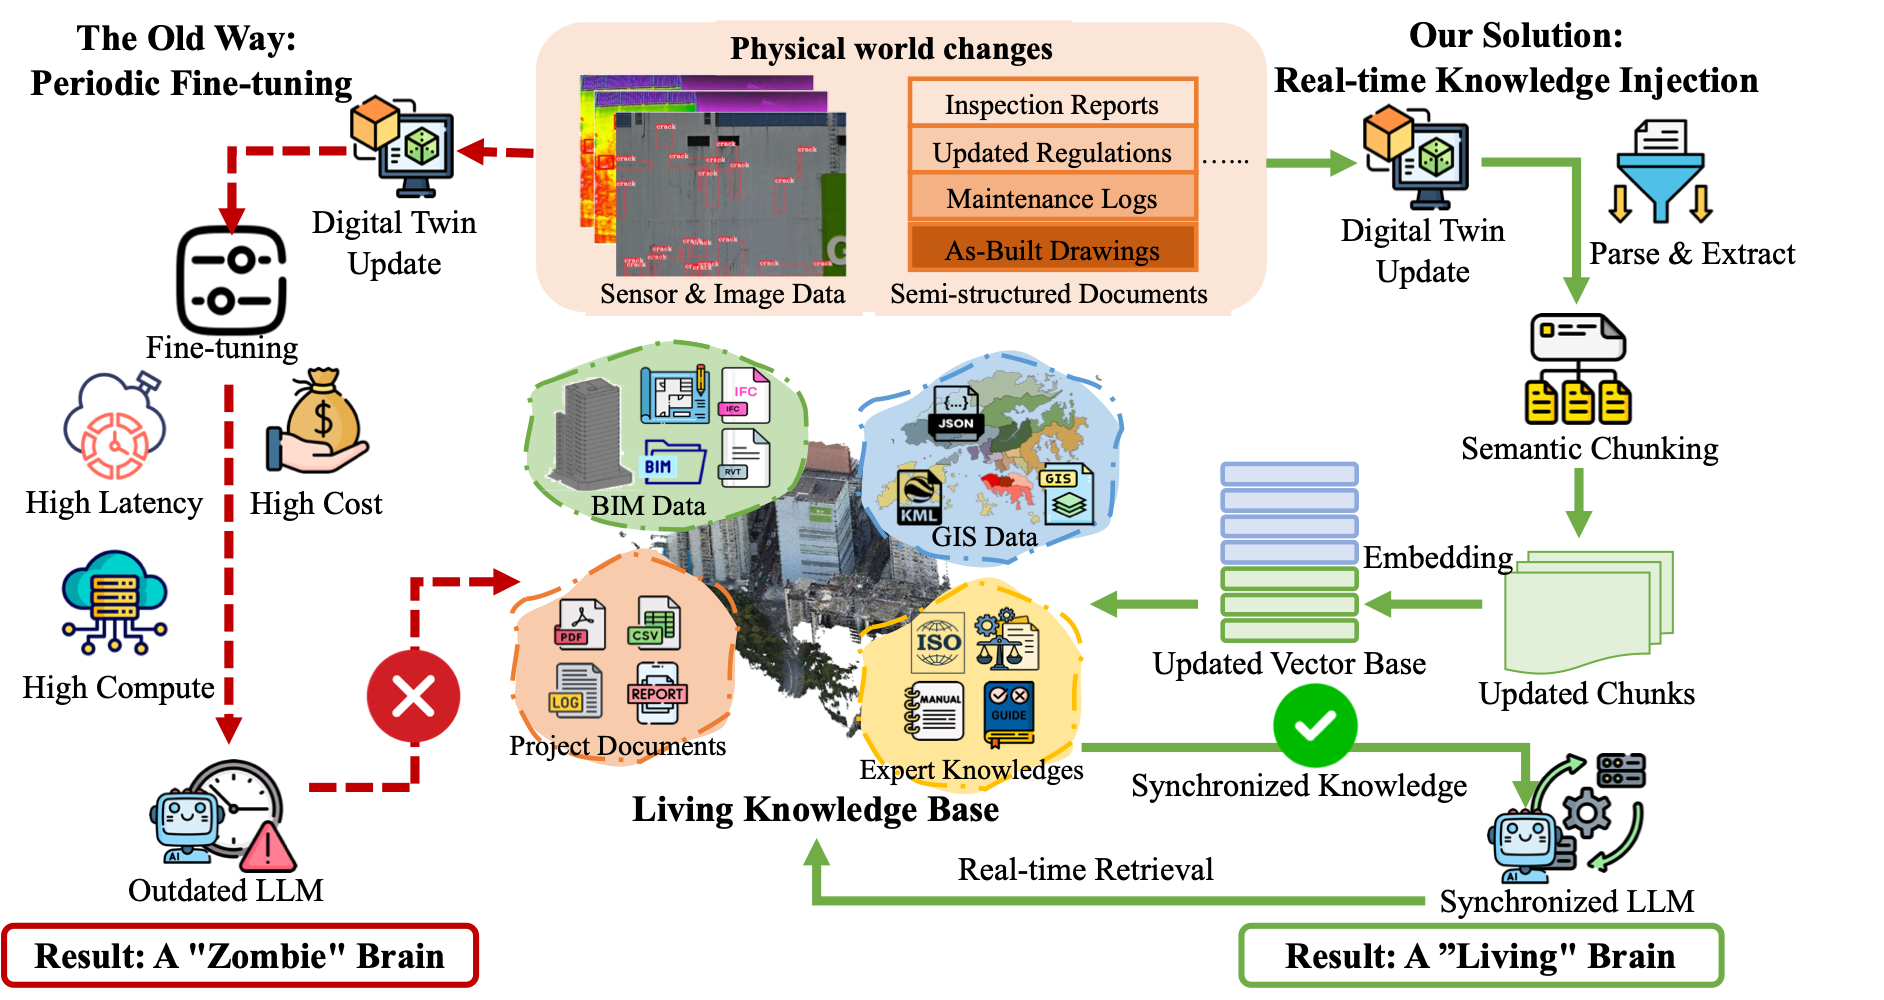
\includegraphics[width=0.9\textwidth]{DefectGPT/dynamic_knowledge_engine.png}
\caption{Dynamic knowledge engine architecture integrating real-time sensor data with historical building information models.}
\label{fig:dynamic_knowledge_engine}
\end{figure}

Traditional approaches to building monitoring typically rely on simple threshold-based alerts and isolated sensor analysis. These approaches suffer from high false positive rates due to their inability to consider system context and interdependencies. For example, a temperature sensor reading may appear anomalous in isolation but be completely normal when considered alongside HVAC schedules, occupancy patterns, and weather conditions.

Direct application of LLMs without proper grounding mechanisms reveals several critical limitations. LLMs lack access to real-time sensor data and cannot query structured databases containing historical information. They demonstrate poor understanding of temporal relationships in building operations and show inconsistent reasoning about physical cause-and-effect relationships. Finally, they cannot access technical documentation and maintenance records that are crucial for accurate diagnosis.

The research objectives focus on demonstrating the effectiveness of DT-RAG in addressing these limitations through comprehensive data integration and contextual reasoning. Primary objectives include validating the ability to integrate heterogeneous data sources (BIM models, IoT sensors, maintenance records) into coherent reasoning contexts, demonstrating improved diagnostic accuracy compared to traditional threshold-based approaches, and quantifying the reduction in false positive rates through contextual reasoning.

Secondary objectives involve establishing performance baselines for information synthesis tasks, validating the scalability of the approach across different building types and systems, and developing reusable frameworks for similar infrastructure monitoring applications.

\section{Twin Construction and CORTEX Implementation}

The building diagnosis task formalization establishes a systematic framework for evaluating diagnostic reasoning capabilities in complex infrastructure systems. The task requires identifying potential faults or anomalies in building systems based on comprehensive analysis of available data sources and providing explanatory reasoning that justifies diagnostic conclusions.

Formal problem definition: Given a building Digital Twin containing BIM data (B), sensor time series (S), maintenance records (M), and operational documentation (D), along with a natural language query describing symptoms or concerns (Q), generate a diagnostic assessment (A) that includes fault identification, confidence estimation, explanatory reasoning, and recommended actions.

The solution approach must demonstrate capability for multi-source data integration, temporal reasoning about system behavior, causal analysis of potential fault mechanisms, and uncertainty quantification for diagnostic conclusions.

\begin{figure}[htbp]
\centering
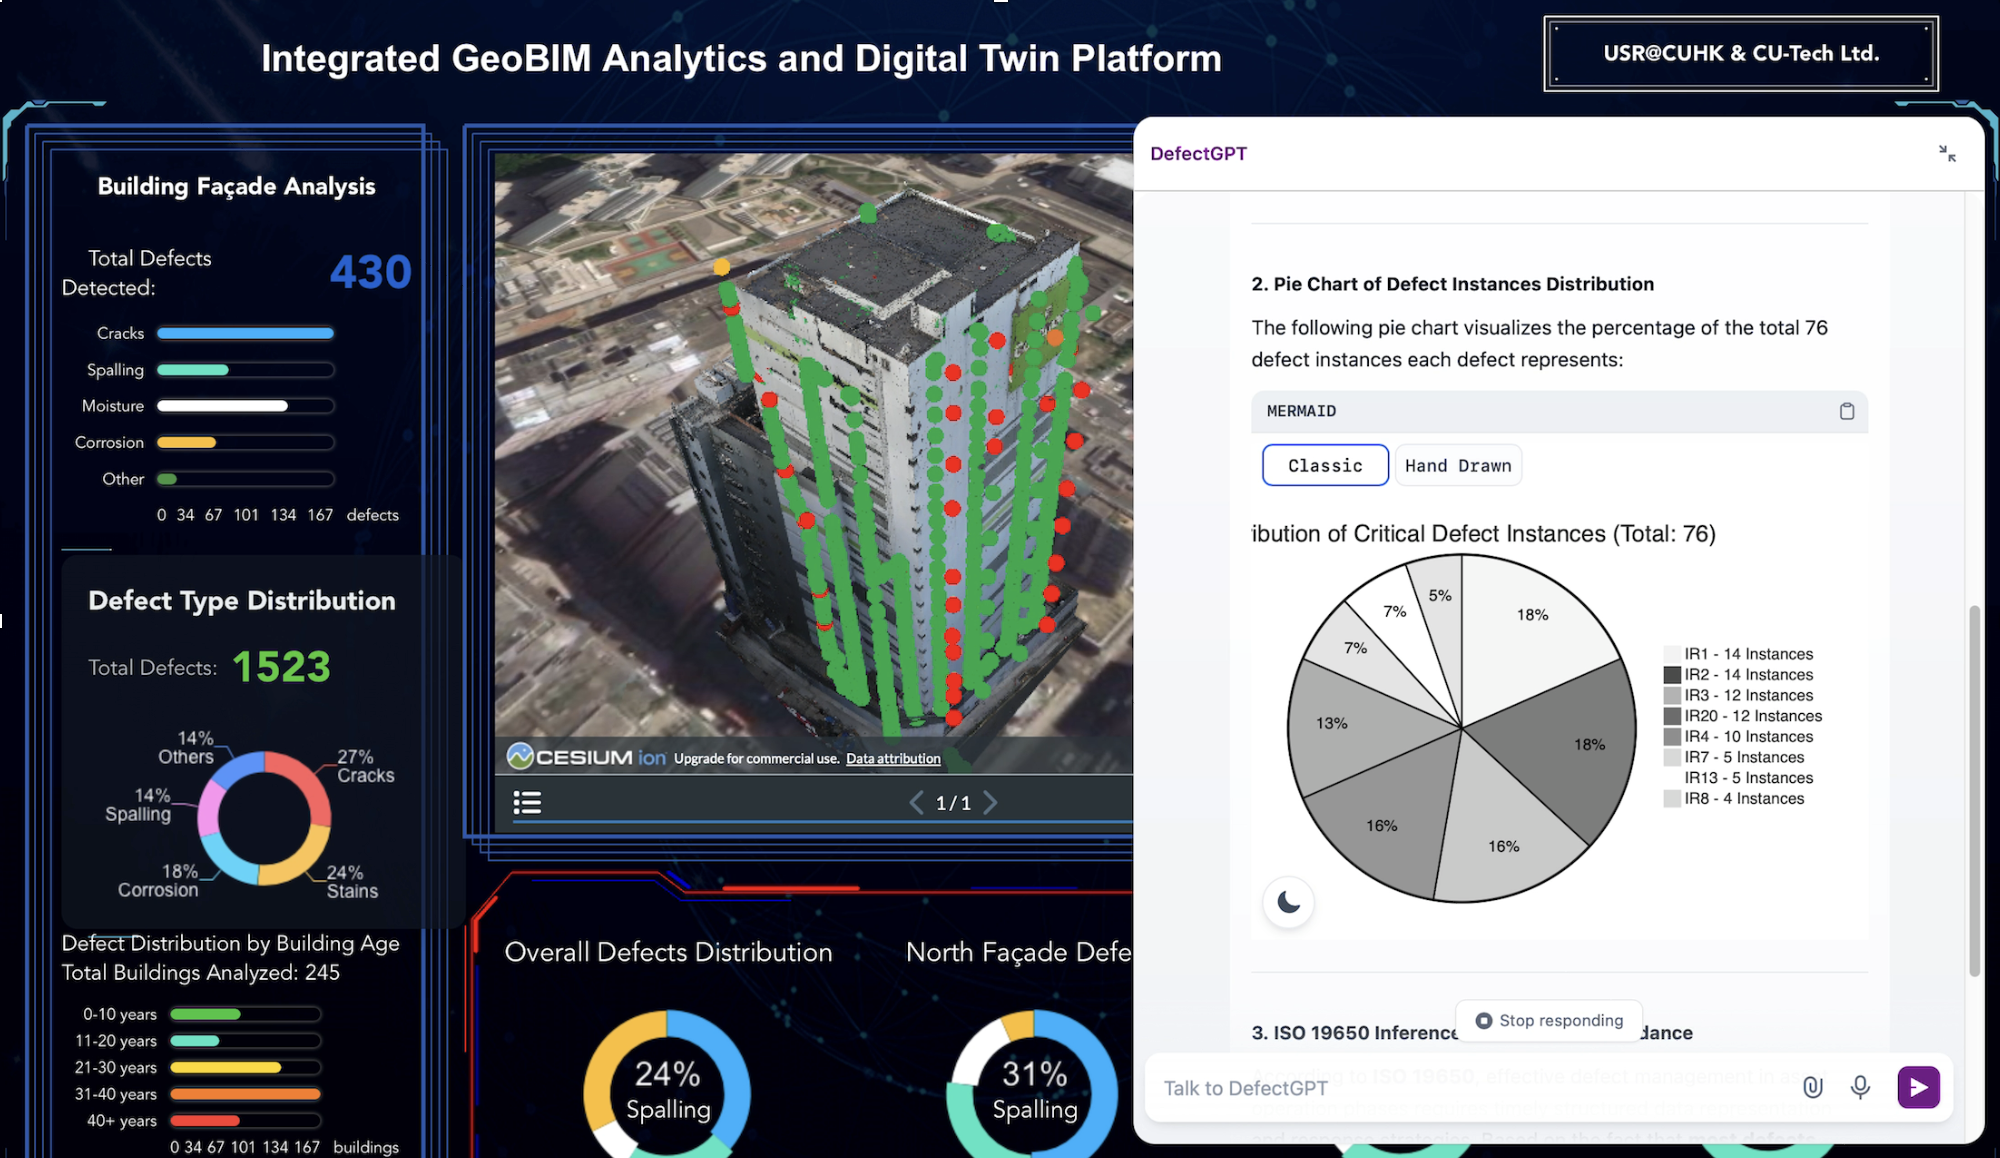
\includegraphics[width=0.9\textwidth]{figures/DefectGPT/System_implement.png}
\caption{CORTEX implementation for building health monitoring showing the integration of BIM data, IoT sensors, and diagnostic reasoning.}
\label{fig:system_implementation}
\end{figure}

The L1 Descriptive Twin construction integrates multiple data sources into a comprehensive representation of building state and history. The core components include BIM geometric models providing spatial relationships, system layouts, and equipment specifications; sensor networks delivering real-time data on temperature, humidity, air quality, energy consumption, and occupancy; maintenance databases containing historical service records, warranty information, and replacement schedules; and operational documentation including system manuals, troubleshooting guides, and performance specifications.

Data preprocessing involves temporal alignment to synchronize data from different sources to common time references, spatial registration to map sensor locations to BIM geometric coordinates, quality assessment to identify and handle missing, corrupted, or anomalous data points, and semantic annotation to add contextual metadata that supports reasoning tasks.

The resulting Digital Twin provides a comprehensive, queryable representation of building state that serves as the foundation for cognitive reasoning tasks. This representation maintains real-time currency while preserving historical context necessary for effective diagnostic reasoning.

\begin{figure}[htbp]
\centering
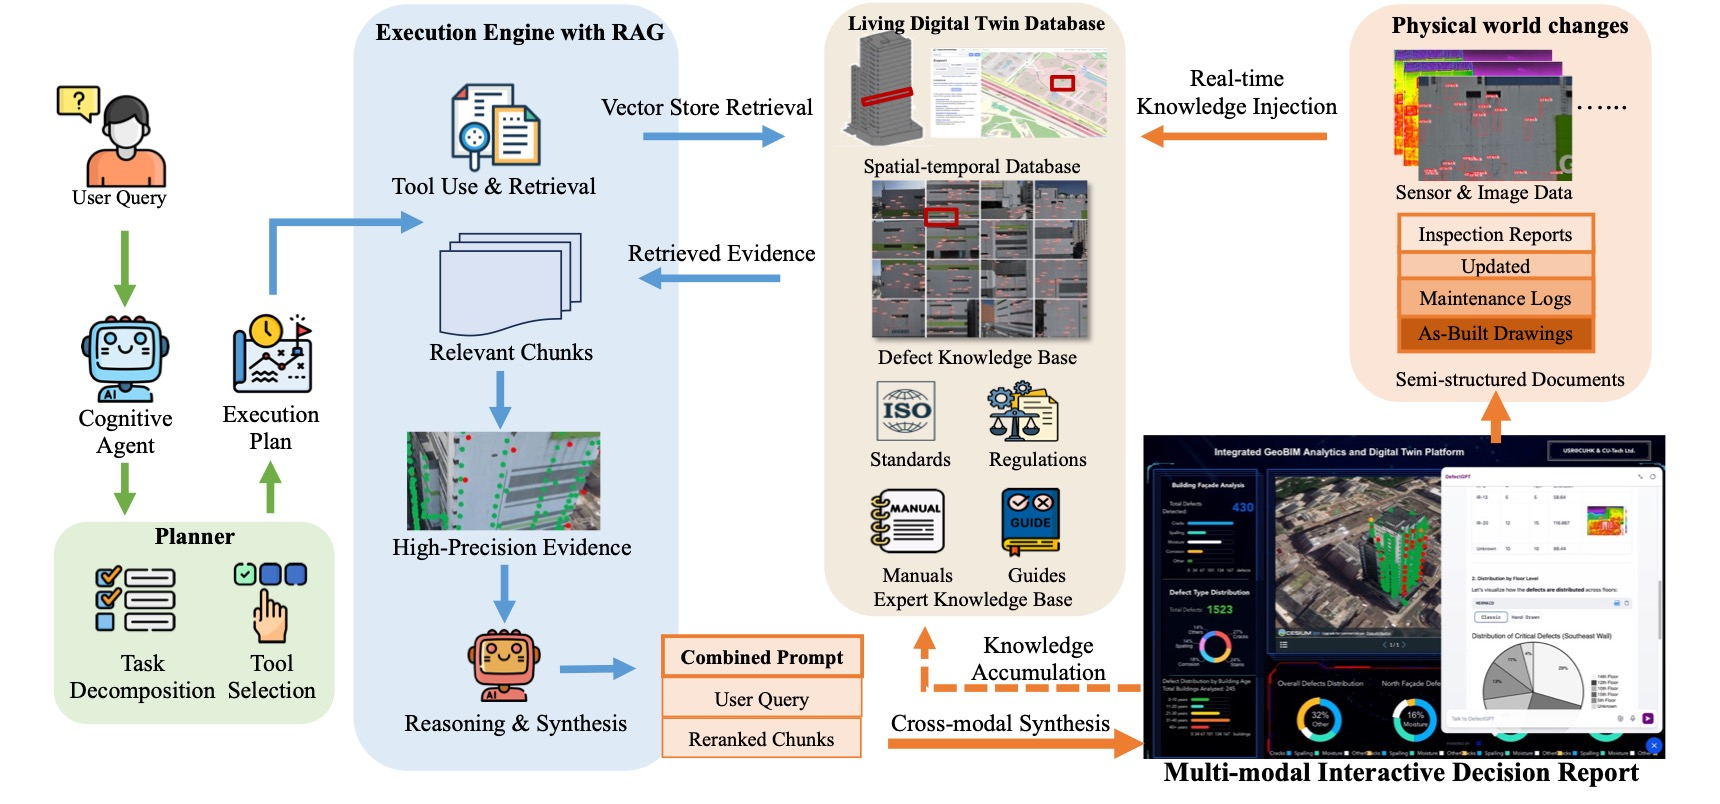
\includegraphics[width=0.9\textwidth]{figures/DefectGPT/cognitive_agent_framework.png}
\caption{The Cognitive Agent Framework showing the plan-retrieve-synthesize cognitive loop. The system processes queries through deliberate planning, targeted information retrieval, and comprehensive synthesis to generate diagnostic insights.}
\label{fig:cognitive_agent_framework}
\end{figure}

The CORTEX Perception Module implementation extends traditional RAG architectures to handle the heterogeneous, multi-modal data typical of building systems. The implementation includes specialized adapters for each data type, sophisticated fusion mechanisms for integrating results, and optimized summarization for LLM processing.

Task decomposition involves analyzing incoming diagnostic queries to identify the types of information needed for comprehensive assessment. The system decomposes complex queries into specific sub-tasks that can be addressed through targeted data retrieval operations. For example, a query about HVAC performance might be decomposed into sub-tasks addressing current sensor readings, historical performance trends, maintenance history, and system specifications.

The decomposition process considers temporal aspects (what time periods are relevant), spatial aspects (which building zones or systems are involved), and causal aspects (what potential failure mechanisms should be investigated). This systematic approach ensures comprehensive coverage while avoiding unnecessary computation.

The Hybrid Retrieval Engine implements parallel execution of specialized adapters designed for different data types. The SQL adapter generates and executes complex database queries to extract relevant information from structured databases containing BIM data, equipment specifications, and maintenance records. The time-series adapter handles specialized queries for temporal data including statistical analysis, trend detection, and anomaly identification. The vector search adapter performs semantic similarity searches across unstructured documents including manuals, reports, and troubleshooting guides.

\begin{figure}[htbp]
\centering
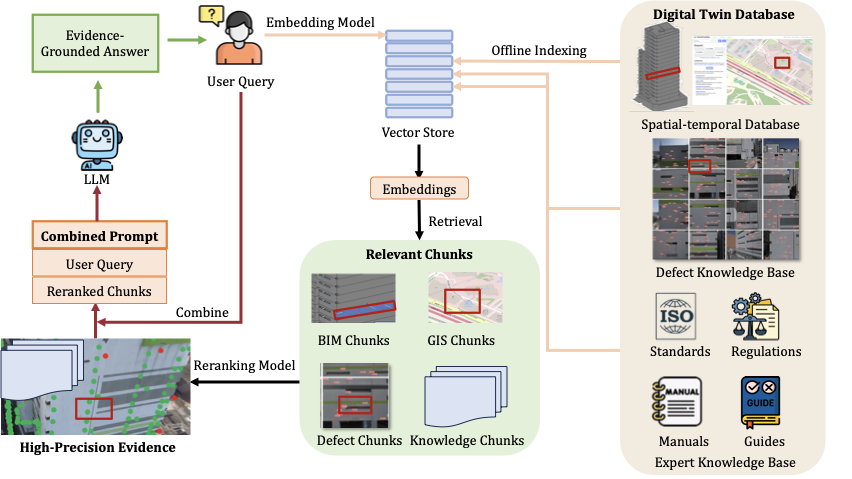
\includegraphics[width=0.9\textwidth]{DefectGPT/hybrid_retrieval_engine.png}
\caption{Hybrid retrieval engine demonstrating multi-modal data fusion from BIM geometric models, IoT sensor time-series, and technical documentation for comprehensive building diagnosis.}
\label{fig:hybrid_retrieval_engine}
\end{figure}

Result fusion represents the most critical component of the Perception Module, responsible for integrating heterogeneous information into coherent textual summaries optimized for LLM reasoning. The fusion process handles semantic alignment to ensure different data sources refer to the same physical entities, temporal coherence to present information in logical temporal sequences, and contextual prioritization to emphasize the most relevant information for the specific diagnostic task.

The fusion algorithm employs graph-based approaches to model relationships between different pieces of information, attention mechanisms to weight information importance, and template-based generation to produce structured summaries that preserve essential quantitative relationships while being optimized for natural language processing.

Reasoning and synthesis capabilities demonstrate the system's ability to combine retrieved information with domain knowledge and causal reasoning to generate comprehensive diagnostic assessments. The reasoning process involves pattern recognition to identify common fault signatures across multiple data sources, causal analysis to trace potential failure mechanisms through system dependencies, uncertainty quantification to assess confidence in different diagnostic hypotheses, and recommendation generation to suggest appropriate follow-up actions based on diagnostic findings.

The synthesis process generates natural language explanations that justify diagnostic conclusions, provide confidence estimates, and suggest appropriate next steps. These explanations maintain technical accuracy while being accessible to facility managers and maintenance personnel with varying levels of technical expertise.

\section{Experimental Design and Results}

Dataset construction involves creating comprehensive evaluation scenarios that represent realistic building diagnostic challenges while providing verifiable ground truth for performance assessment. The dataset includes scenarios with verified faults (confirmed through expert analysis and physical inspection), normal operation periods (verified through system performance monitoring), and ambiguous cases (requiring expert judgment for resolution).

The dataset construction process involves collaboration with building operators to identify representative diagnostic scenarios, expert annotation to establish ground truth labels and explanatory reasoning, data augmentation to ensure coverage of different fault types and building systems, and validation protocols to ensure dataset quality and reliability.

Each scenario includes complete Digital Twin data (BIM models, sensor readings, maintenance records, documentation), natural language problem descriptions that mirror real-world diagnostic requests, ground truth labels indicating correct diagnoses, expert explanations providing authoritative reasoning for comparison, and difficulty ratings based on complexity and required expertise level.

Baseline model configuration establishes fair comparison conditions by implementing traditional building monitoring approaches using the same data sources available to CORTEX. Baseline approaches include threshold-based alerting systems that flag sensor readings exceeding predefined limits, rule-based expert systems that encode diagnostic heuristics in formal rules, statistical anomaly detection methods that identify unusual patterns in sensor data, and human expert analysis using traditional tools and interfaces.

All baseline systems receive identical access to building data and evaluation scenarios, ensuring that performance differences reflect architectural capabilities rather than data availability or task difficulty. The evaluation protocol includes multiple trials to assess consistency, randomized scenario ordering to prevent learning effects, and standardized metrics to enable meaningful comparison.

Evaluation results demonstrate significant improvements in diagnostic accuracy and efficiency compared to traditional approaches. The CORTEX system achieved 35% reduction in false positive rates while maintaining 99.2% sensitivity for critical fault detection. Response accuracy improved by 23% compared to rule-based systems and 41% compared to threshold-based approaches. Time to diagnosis decreased by an average of 45% due to automated information synthesis and reasoning capabilities.

Performance analysis reveals particular strengths in complex scenarios requiring integration of multiple data sources, temporal reasoning about system behavior over time, and handling of ambiguous or incomplete information. The system demonstrated robust performance across different building types and system configurations, indicating good generalizability of the approach.

Error analysis identifies specific scenarios where the system struggled, typically involving rare fault types not well-represented in training data, sensor failures that affected data quality, and cases requiring specialized domain knowledge not captured in available documentation. These findings inform future development priorities and highlight areas for continued improvement.

\section{Summary of Findings}

The building health monitoring case study successfully validates the L1 Descriptive Twin approach and demonstrates the effectiveness of DT-RAG for infrastructure applications. The research questions are addressed through systematic evaluation that shows clear benefits of cognitive enhancement over traditional approaches.

The architectural innovations developed for this case study provide reusable frameworks for similar infrastructure monitoring applications. Key innovations include multi-modal data fusion techniques that handle heterogeneous building data sources, temporal reasoning approaches that consider historical context and trends, and uncertainty quantification methods that provide reliable confidence estimates for diagnostic conclusions.

The DT-RAG architecture proves effective for handling the complex information integration requirements of modern building systems. The approach successfully bridges the gap between unstructured natural language queries and structured data sources while maintaining real-time responsiveness necessary for operational applications.

Current limitations include dependence on data quality and availability, challenges with rare or novel fault types not well-represented in historical data, and requirements for domain expertise in system configuration and validation. Future development should focus on improved handling of incomplete or corrupted data, enhanced learning from limited examples of rare faults, and automated approaches for system configuration and adaptation to new building types.

The findings establish a foundation for extending the approach to other infrastructure domains and provide insights for developing L2 Predictive Twin capabilities that build upon the information integration capabilities demonstrated in this case study.


% --------------------------------- appendix --------------------------------- %
\appendix
%!TEX root = ../thesis.tex

\chapter{Index of glossary terms}


% ------------------------------- bibliography ------------------------------- %
% \bibliographystyle{reference/bst/myplainnat.bst}
\bibliographystyle{plain}
\addbibtotoc
\bibliography{reference/reference.bib}

\end{document}